\X{To satisfy the C2 agility requirements and in line with Self-Adaptive Systems (SAS)~\citep{AlvesSBBG09}, our proposal relies on the software capacity of adapting to deal with requirements change in runtime. Relying on different valid products generation from a common artifact set, just activating or deactivating features, to provide context dealing, the Software Product Line (SPL) approach~\citep{SPL_SAS01}, extended to dynamic scenarios, shows itself is a suitable choice for dealing with such a variability. Based on this, we leverage Dynamic Software Product Line (DSPL) as a strategy for implementing this capability of runtime reconfiguration.} 

\X{Performance is not in this work’s scope and it makes DSPL a workable strategy to deal with varying requirements and constraints as a SAS approach~\citep{SPL_SAS01}. Based on this, we combine such a definition to present a computational model capable of representing the scenario members’ behaviors based on the roles that such elements have.}

To cope with context changes, the members, modeled as DSPL, may reconfigure themselves or adjust their coordination according to the communication structure and information exchange of a C2 strategy. This capacity is enabled by a model that allows coordination and data exchange via so called channels, and a member’s description composed by features that can be dynamically enabled according to the circumstances, generating different configurations. Particularly, the proposed computational model is a typed-parameterized extension of the channel system presented in Section~\ref{ssec:background_cs}, henceforth referred to as C2 channel system (C2CS), which is described \X{in the next} sections.

%To provide C2 Agility, the proposal is to present a computational model capable of representing the scenario members’ behaviors based on the roles that such elements have. To cope with context changes, these members may reconfigure themselves or adjust their coordination according to the communication structure and information exchange of a C2 strategy. This capacity is enabled by a model that allows coordination and data exchange via so called channels, and a member’s description composed by features that can be dynamically enabled according to the circumstances, generating different configurations. Particularly, the proposed computational model is a typed-parameterized extension of the channel system presented in Section~\ref{ssec:background_cs}, henceforth referred to as C2 channel system (C2CS), which is described \X{in the next} sections.



\subsection{Typed-Parameterized Channel System}
\label{sec:channelSystem}

Essentially, C2CS defines coordination among entities and their reconfiguration to cope with context changes eventually arising during a mission. These behaviors are described by three different program graphs (PGs) making up C2CS and representing role types played by entities: \textit{Task Performer (TP)}, \textit{Task Allocator (TA)}, and \textit{C2 Approach Manager (C2AM)}. TP establishes the tasks' execution and entity's reconfiguration behavior. TA defines task allocation responsibilities among entities, and C2AM specifies a C2 Approach change protocol. Types are used to describe the structure of the PG's locations as well as of the message content exchanged in synchronous and asynchronous channels. 

Figure \ref{fig:cs} depicts C2CS, whereas Equation~\ref{eq:cs} defines it. The use of channel system concepts allows the execution of parallel processes with communication capability among them. Such a structure allows us to model the identified roles in a C2 system running in parallel and performing information exchange. This exchange leverages channels, i.e., first-in, first-out buffers that carry messages. The C2CS employs both synchronous and asynchronous channels. The former, e.g., $ch_2$ and $ch_3$, synchronizes C2AM's and TA's PG when they perform tasks allocation and C2 Approach change. The latter, e.g., $m_k$ and $ch_1$, enables the transmission of allocated tasks to the TPs and the return of not possible tasks to the TA. 

\begin{figure}[ht]
    \centering
    \scalebox{.8}{

\tikzset{every picture/.style={line width=0.75pt}} %set default line width to 0.75pt        

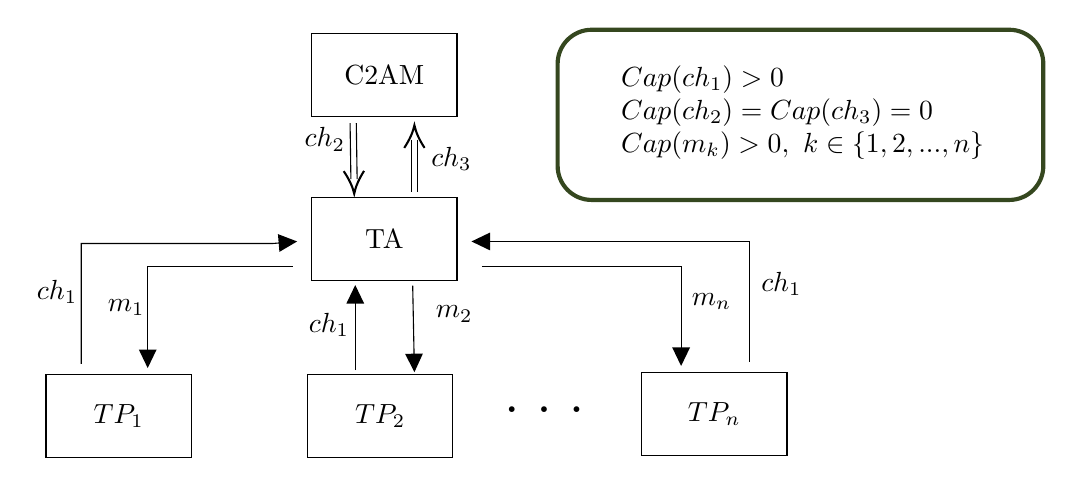
\begin{tikzpicture}[x=0.75pt,y=0.75pt,yscale=-1,xscale=1]
%uncomment if require: \path (0,225); %set diagram left start at 0, and has height of 225

%Shape: Rectangle [id:dp7793135649662085] 
\draw   (146,89) -- (216,89) -- (216,129) -- (146,129) -- cycle ;
%Shape: Rectangle [id:dp8388066725390221] 
\draw   (146,10) -- (216,10) -- (216,50) -- (146,50) -- cycle ;
%Shape: Rectangle [id:dp48691256180587716] 
\draw   (18,174) -- (88,174) -- (88,214) -- (18,214) -- cycle ;
%Straight Lines [id:da7136052167478543] 
\draw    (194.67,131.33) -- (195.44,170) ;
\draw [shift={(195.5,173)}, rotate = 268.85] [fill={rgb, 255:red, 0; green, 0; blue, 0 }  ][line width=0.08]  [draw opacity=0] (8.93,-4.29) -- (0,0) -- (8.93,4.29) -- cycle    ;
%Straight Lines [id:da1199439366931846] 
\draw    (35,169) -- (35,111) -- (127,111) -- (136.01,110.25) ;
\draw [shift={(139,110)}, rotate = 535.24] [fill={rgb, 255:red, 0; green, 0; blue, 0 }  ][line width=0.08]  [draw opacity=0] (8.93,-4.29) -- (0,0) -- (8.93,4.29) -- cycle    ;
%Shape: Rectangle [id:dp8070909053866772] 
\draw   (305,173) -- (375,173) -- (375,213) -- (305,213) -- cycle ;
%Shape: Rectangle [id:dp18131918632628874] 
\draw   (144,174) -- (214,174) -- (214,214) -- (144,214) -- cycle ;
%Straight Lines [id:da23459308482895536] 
\draw    (357,168) -- (357,110) -- (226,110) ;
\draw [shift={(223,110)}, rotate = 360] [fill={rgb, 255:red, 0; green, 0; blue, 0 }  ][line width=0.08]  [draw opacity=0] (8.93,-4.29) -- (0,0) -- (8.93,4.29) -- cycle    ;
%Straight Lines [id:da9340034396500284] 
\draw    (228,122) -- (324,122) -- (324,167) ;
\draw [shift={(324,170)}, rotate = 270] [fill={rgb, 255:red, 0; green, 0; blue, 0 }  ][line width=0.08]  [draw opacity=0] (8.93,-4.29) -- (0,0) -- (8.93,4.29) -- cycle    ;
%Straight Lines [id:da26523318096149495] 
\draw    (137,122) -- (67,122) -- (67,168) ;
\draw [shift={(67,171)}, rotate = 270] [fill={rgb, 255:red, 0; green, 0; blue, 0 }  ][line width=0.08]  [draw opacity=0] (8.93,-4.29) -- (0,0) -- (8.93,4.29) -- cycle    ;
%Straight Lines [id:da6224238934860249] 
\draw    (167,172) -- (167,134) ;
\draw [shift={(167,131)}, rotate = 450] [fill={rgb, 255:red, 0; green, 0; blue, 0 }  ][line width=0.08]  [draw opacity=0] (8.93,-4.29) -- (0,0) -- (8.93,4.29) -- cycle    ;
%Straight Lines [id:da30878293142018354] 
\draw    (167.5,52.98) -- (167.9,79.98)(164.5,53.02) -- (164.9,80.02) ;
\draw [shift={(166.5,87)}, rotate = 269.15999999999997] [color={rgb, 255:red, 0; green, 0; blue, 0 }  ][line width=0.75]    (10.93,-4.9) .. controls (6.95,-2.3) and (3.31,-0.67) .. (0,0) .. controls (3.31,0.67) and (6.95,2.3) .. (10.93,4.9)   ;
%Straight Lines [id:da1036410124215259] 
\draw    (197,61) -- (197,86)(194,61) -- (194,86) ;
\draw [shift={(195.5,54)}, rotate = 90] [color={rgb, 255:red, 0; green, 0; blue, 0 }  ][line width=0.75]    (10.93,-4.9) .. controls (6.95,-2.3) and (3.31,-0.67) .. (0,0) .. controls (3.31,0.67) and (6.95,2.3) .. (10.93,4.9)   ;
%Rounded Rect [id:dp17275257935630328] 
\draw  [color={rgb, 255:red, 53; green, 71; blue, 31 }  ,draw opacity=1 ][line width=1.5]  (264.5,24.4) .. controls (264.5,15.34) and (271.84,8) .. (280.9,8) -- (482.1,8) .. controls (491.16,8) and (498.5,15.34) .. (498.5,24.4) -- (498.5,73.6) .. controls (498.5,82.66) and (491.16,90) .. (482.1,90) -- (280.9,90) .. controls (271.84,90) and (264.5,82.66) .. (264.5,73.6) -- cycle ;

% Text Node
\draw (181,30) node   [align=left] {C2AM};
% Text Node
\draw (181,109) node   [align=left] {TA};
% Text Node
\draw (53,194) node    {$TP_{1}$};
% Text Node
\draw (23.33,134.33) node    {$ch_{1}$};
% Text Node
\draw (214.67,145) node    {$m_{2}$};
% Text Node
\draw (340,193) node    {$TP_{n}$};
% Text Node
\draw (179,194) node    {$TP_{2}$};
% Text Node
\draw (258,191) node  [font=\Large] [align=left] {\textbf{. . .}};
% Text Node
\draw (338.67,139) node    {$m_{n}$};
% Text Node
\draw (56.67,142) node    {$m_{1}$};
% Text Node
\draw (154.33,150.33) node    {$ch_{1}$};
% Text Node
\draw (372.33,130.33) node    {$ch_{1}$};
% Text Node
\draw (152.33,60.83) node    {$ch_{2}$};
% Text Node
\draw (213.33,70.33) node    {$ch_{3}$};
% Text Node
\draw (382.5,48) node    {$ \begin{array}{l}
Cap( ch_{1})  >0\\
Cap( ch_{2}) =Cap( ch_{3}) =0\\
Cap( m_{k})  >0,\ k\in \{1,2,...,n\}
\end{array}$};


\end{tikzpicture}}
    \caption{C2 Channel System for a team composed by \textit{n} members with the TP role asynchronous and synchronous channels represented by single and double line arrows, respectively.}
    \label{fig:cs}
\end{figure}


\begin{equation}
    \label{eq:cs}
    \begin{split}
    C2CS([FM]\ E,\ &  \mathcal{P}(Task)\ M,\ C2_{ap}\ \omega_0) = [C2AM(E, M,\omega_0)\ |\ TA\ | \\ & \ TP(fm_1, \omega_0)\ |\ ...\ |\ TP(fm_n, \omega_0)]
    \end{split}
\end{equation}

\color{black}
In Equation~\ref{eq:cs}, the parameters have the following meaning and types. The set $M=\{t_1, t_2,\ ...,\ t_m \}$ is the designated mission, consisting of tasks that the members will try to perform. $M$ belongs to $\mathcal{P}(Task)$, which is the power set of $Task$, where $Task=\{t_a, t_b,\ ...,\ t_z \}$ is the set of all possible tasks. The list $E = [fm_1, fm_2,\ ...,\ fm_n ]$ of team members is such that each team member has a capability of type Feature Model ($FM$). Additionally, such members always operate a C2 Approach $\omega \in \Omega$, where $\Omega =$ \textit{\{Edge, Collaborative, Coordinated, De-Conflicted, Conflicted\}}. Lastly, the vertical bars represent parallel composition of the PGs representing the roles played by the team members.
\color{black}

C2CS leverages parameters to abstract from specific mission, entities, and initial conditions. It models roles that will be performed by the agents.

Each role played by the entities is represented by a PG that receives parameters that define some aspects of its internal structure. Such PGs are parallel processes that compose the C2CS and are instantiated according to the C2 Approach selected. Instances of different PGs can coexist in the same member according to the C2 Approach operated. In particular, the representation of multiple TPs shown in Figure~\ref{fig:cs} is to emphasize the existence of a specific asynchronous channel $m_k$ for each member $k$ owning a TP role instance, from where they receive the tasks to be performed. All members within $E$ with such a role instance are responsible for the mission's tasks accomplishment. Based on this, the member-to-role-instance mapping is such that each team member may eventually play one instance of the TP, TA, and C2AM roles simultaneously, and more details related to the implementation of this mapping are available in a public repository\footnote{\gitRepository}.
   
 
%The member-to-role-instance mapping is such that each team member plays each EX role instance, and it contributes \textit{partially} to both the TA and the C2A roles, the amount of such contribution depending on the current C2 approach. Conversely, each EX role instance is cohesively encapsulated in one member, whereas the C2A and the TA roles are \textit{scattered} throughout team members, given the inherent collaborative nature of these roles.  it.
%Team members contribute to all roles with dynamic intensity during the mission. 

In a typical C2CS scenario, when the mission starts, TA allocates tasks to team members, which work on accomplishing them. Eventually, to handle context changes, members may reconfigure themselves, e.g., due to sensor failure, or \color{black}the TA \color{black} can reallocate tasks among members, e.g., due to member failure. Alternatively, even a task allocation might not suffice, in which case the C2AM might change the C2 approach, prompting new task allocation among members. \color{black}In the worst scenario, when changing the C2 approach does not suffice, the task fails.\color{black} 


Recalling the motivating example (Section~\ref{sec:example}), in that specific C2 approach the coordinator plays the C2AM and TA roles. Each one of the other members plays the TP role. In that particular case, the loss of one member will first prompt the leader to reallocate tasks to the other team members, using the channels depicted in Figure \ref{fig:example2-a}. 
 Since the only member capable of executing the task that was previously allocated to the lost member is the leader, the C2AM changes the current C2 approach to Edge \citep{FRANCE2014}, prompting this modification using the communication network among members, i.e., the C2 Approach. This way, the former leader now plays the TP role and thus can execute the aforementioned tasks. This resulting situation is illustrated in Figure \ref{fig:example2-b}.

\begin{figure}[!htbp]
	\centering
	\begin{subfigure}[t]{.45\textwidth}
	\centering
	    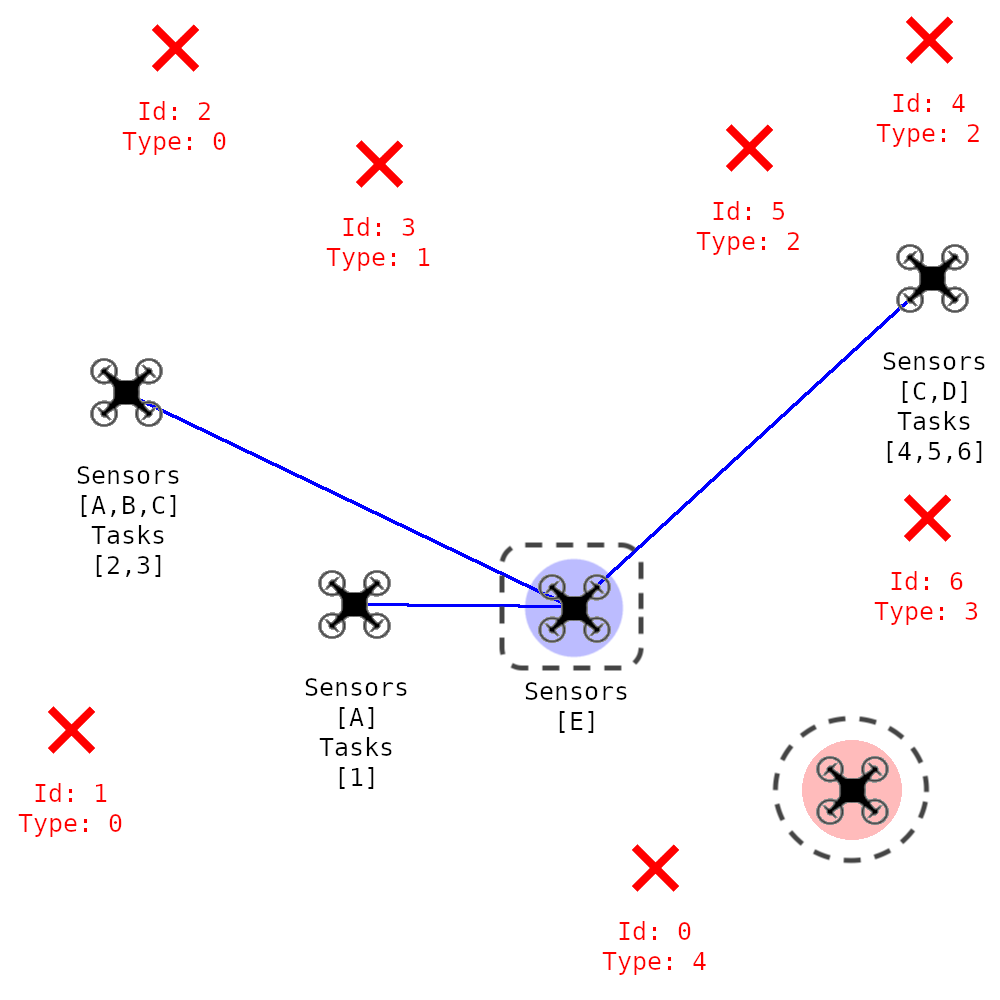
\includegraphics[width=0.95\linewidth]{img/C2Drones2-V4-dashed.png}
	    \caption{UAV dropped (dashed circle)\label{fig:example2-a}}
	\end{subfigure}
	\begin{subfigure}[t]{.45\textwidth}
	\centering
	    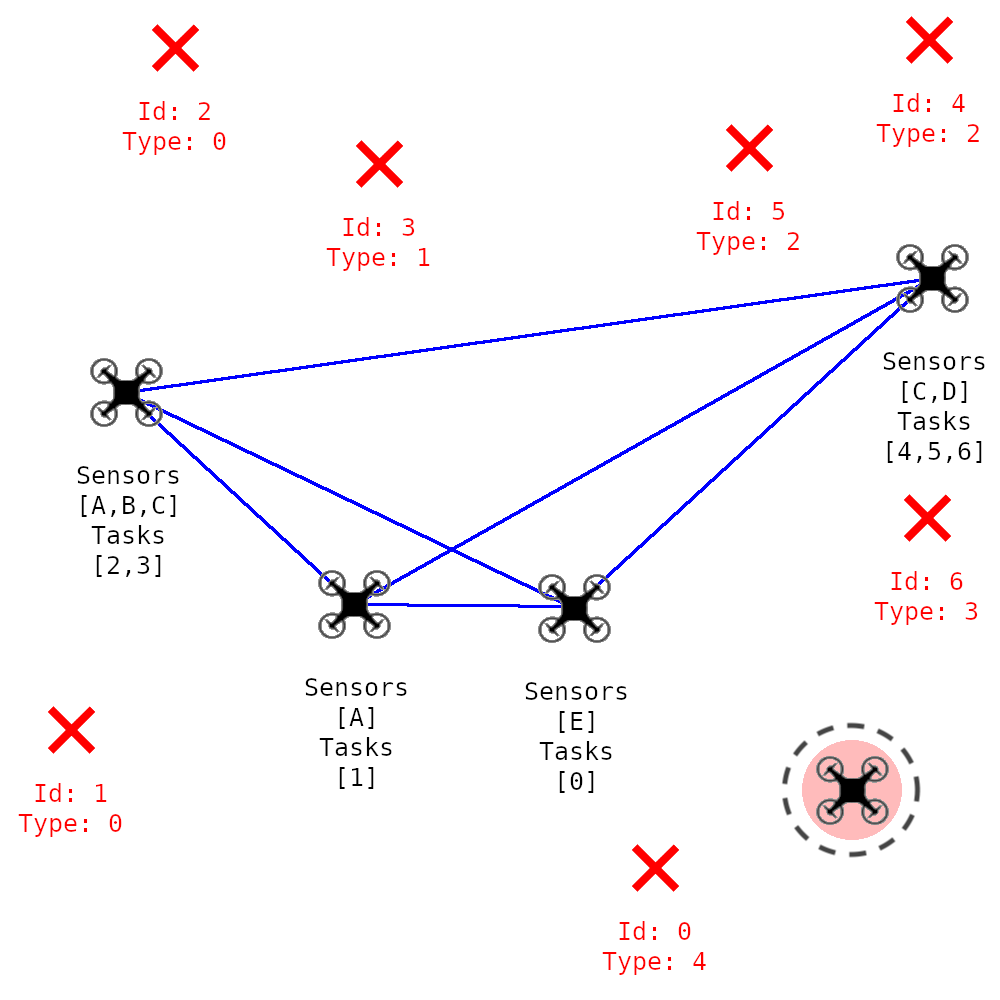
\includegraphics[width=0.95\linewidth]{img/C2Drones3-V4-dashed.png}
	    \caption{C2 Approach change \label{fig:example2-b}}
	\end{subfigure}
	\caption{The team performing tasks after C2 Approach change (lines indicating communication links) due to problems with one of the members (dropped UAV marked with a dashed circle)}
	\label{fig:TeamExecutionAfterManuever}
\end{figure}

% \begin{figure}
% \centering
% \fbox{
% \begin{minipage}{.45\textwidth}
% %\captionsetup{type=figure}
%   \centering
%   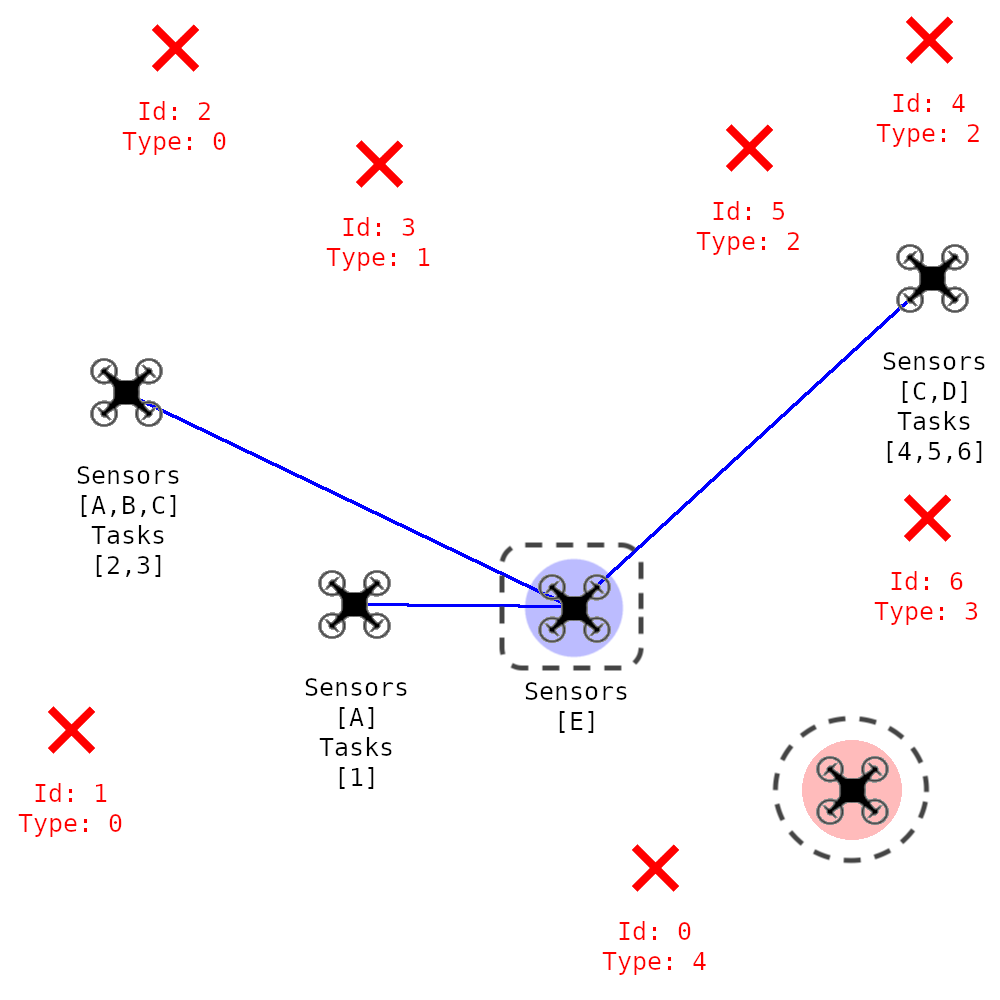
\includegraphics[width=0.95\linewidth]{img/C2Drones2-V4-dashed.png}
%   \subcaptionbox{(a) UAV dropped (dashed circle)\label{fig:example2-a}}{}
% \end{minipage}}%
% \fbox{
% \begin{minipage}{.45\textwidth}
%   \centering
%   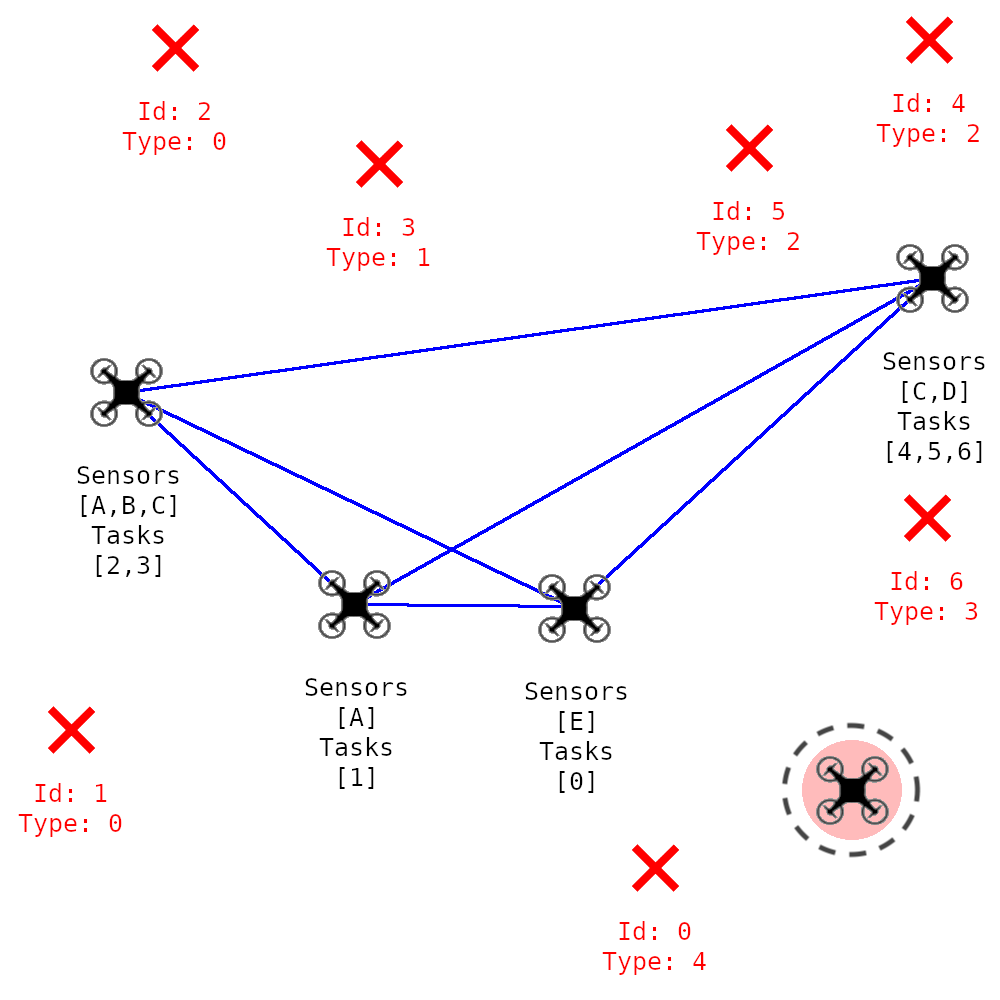
\includegraphics[width=0.95\linewidth]{img/C2Drones3-V4-dashed.png}
%   \subcaptionbox{(b) C2 Approach change \label{fig:example2-b}}{}
% \end{minipage}}
% \caption{The team performing tasks after C2 Approach change (lines indicating communication links) due to problems with one of the members (dropped UAV marked with a dashed circle)}
% \label{fig:example}
% \end{figure}


%\begin{figure}[ht]
%    \centering
%    \fbox{
%    \begin{minipage}{.45\textwidth}
%  \centering
%  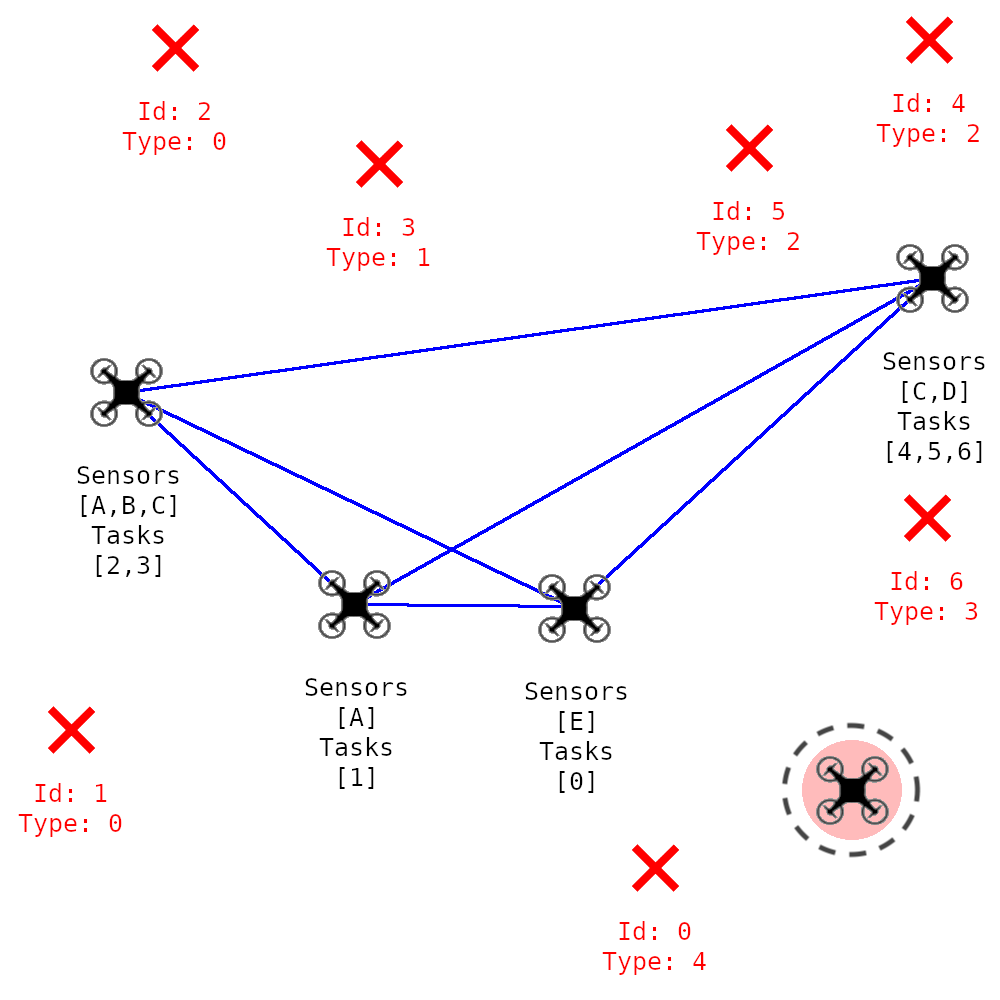
\includegraphics[width=0.95\linewidth]{img/C2Drones3-V4-dashed.png}
%\end{minipage}}
%\caption{The team performing tasks after C2 Approach change(lines indicating communication) due to problems with one of the members(marked with a dashed circle)}
%\label{fig:3TeamExecutionAfterManuever}
%\end{figure}

Overall, reconfiguration, performing new task allocation, and changing the C2 approach under certain context changes are explicitly represented in the PGs, \color{black}thereby enabling the C2CS's strategy \color{black} to achieve agility (cf. Section~\ref{sec:example}). The PGs are detailed in the following, and their implementation is publicly available elsewhere.\footnote{\implementation}

\X{In summary, Figure~\ref{fig:diagram} shows the interaction between these roles played by the members. The tasks received by the member with the role \emph{C2AM} causes an initial C2 approach selection, followed by the members, i.e., DSPL, notification. Next, the \emph{TA} role receives the tasks and performs the allocation. In case of no suitable allocation, the system tries to change the C2 approach to improve the awareness. All allocated tasks are sent to the related TP. This member tries to find a suitable configuration. If it is not possible, the task is reallocated. Finally, with the context changes, the \emph{TA} and the \emph{TP} roles try to adjust themselves. A new configuration is the first deal, followed by the task reallocation. In case they do not work, a new C2 approach is evaluated to obtain a suitable system awareness.
}

\begin{figure}[!ht]
    \centering
    \scalebox{.75}{

\tikzset{every picture/.style={line width=0.75pt}} %set default line width to 0.75pt        

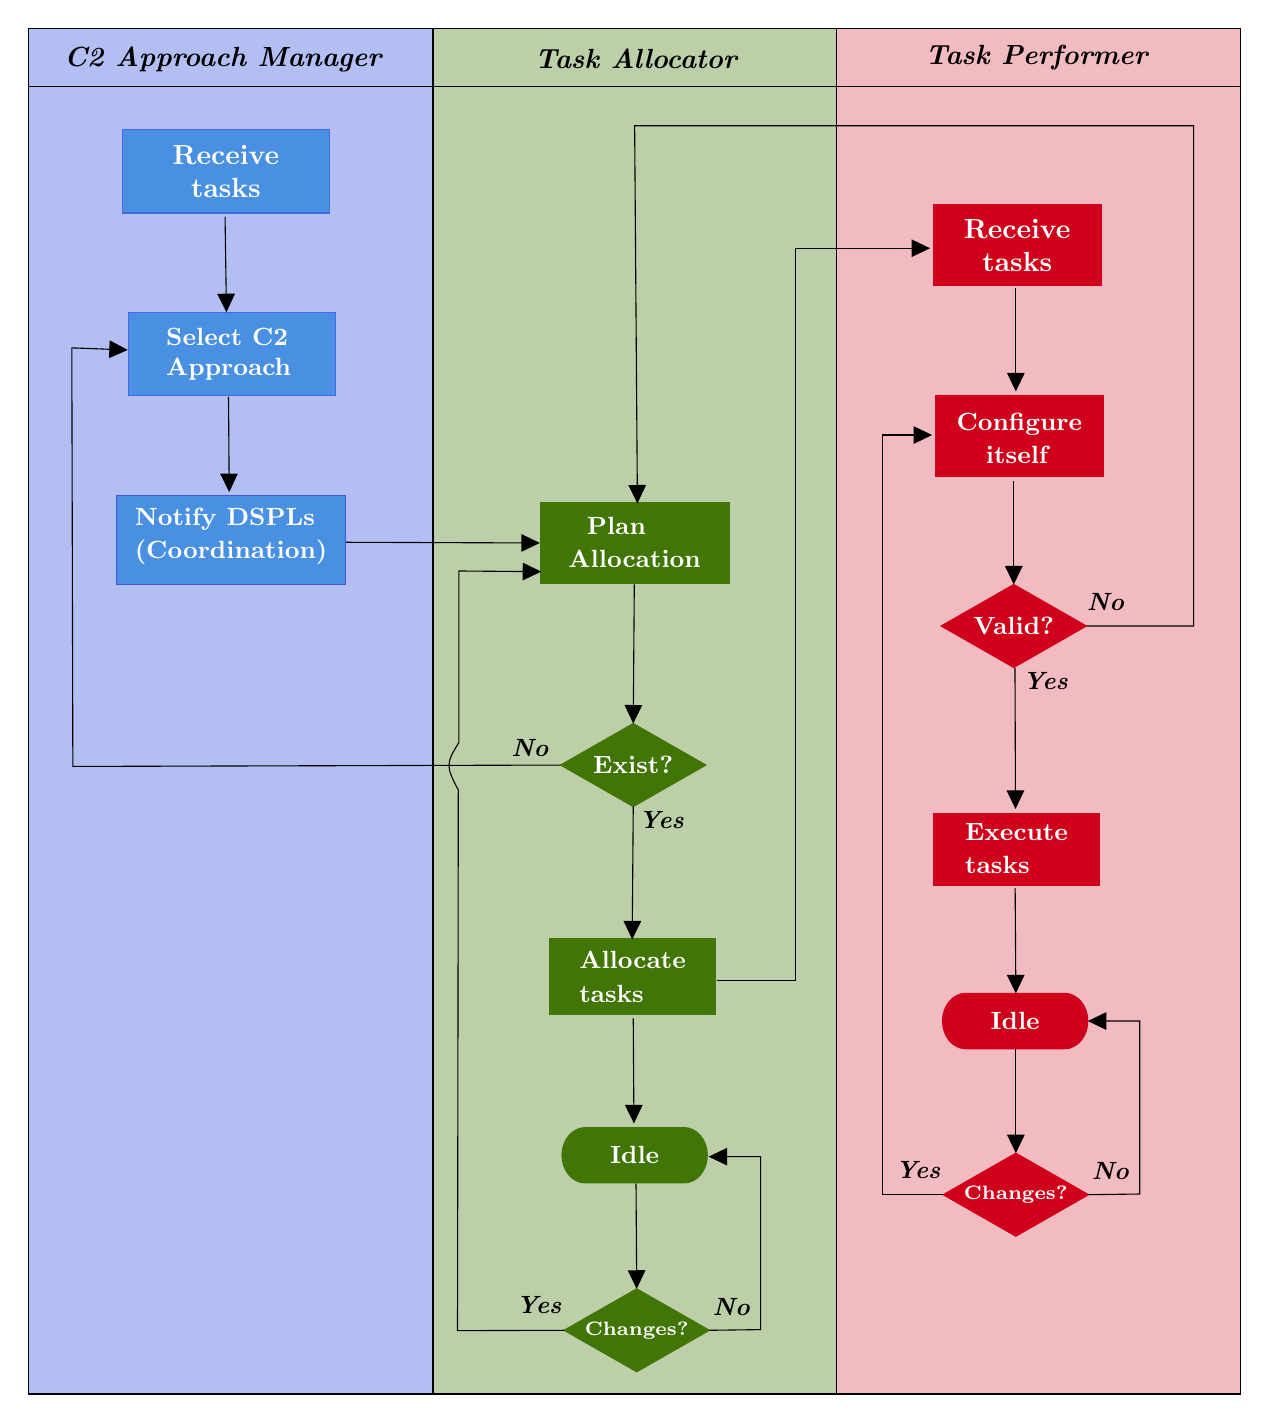
\begin{tikzpicture}[x=0.75pt,y=0.75pt,yscale=-1,xscale=1]
%uncomment if require: \path (0,673); %set diagram left start at 0, and has height of 673

%Shape: Rectangle [id:dp8854253159391561] 
\draw  [fill={rgb, 255:red, 74; green, 102; blue, 226 }  ,fill opacity=0.42 ] (2.5,3) -- (197.5,3) -- (197.5,661) -- (2.5,661) -- cycle ;
%Shape: Rectangle [id:dp3469463448197052] 
\draw  [fill={rgb, 255:red, 65; green, 117; blue, 5 }  ,fill opacity=0.35 ] (197.5,3) -- (392,3) -- (392,661) -- (197.5,661) -- cycle ;
%Shape: Rectangle [id:dp018917795120609204] 
\draw  [fill={rgb, 255:red, 208; green, 2; blue, 27 }  ,fill opacity=0.27 ] (392,3) -- (586.67,3) -- (586.67,661) -- (392,661) -- cycle ;
%Straight Lines [id:da8146359528310543] 
\draw    (2.5,31) -- (587,31) ;
%Flowchart: Process [id:dp15412574148578628] 
\draw  [color={rgb, 255:red, 74; green, 104; blue, 226 }  ,draw opacity=1 ][fill={rgb, 255:red, 74; green, 144; blue, 226 }  ,fill opacity=1 ] (51,140) -- (150.5,140) -- (150.5,180) -- (51,180) -- cycle ;
%Flowchart: Process [id:dp48065105856176205] 
\draw  [color={rgb, 255:red, 74; green, 83; blue, 226 }  ,draw opacity=1 ][fill={rgb, 255:red, 74; green, 144; blue, 226 }  ,fill opacity=1 ] (45,228.17) -- (155.5,228.17) -- (155.5,270.83) -- (45,270.83) -- cycle ;
%Flowchart: Process [id:dp6629894570275567] 
\draw  [color={rgb, 255:red, 65; green, 117; blue, 5 }  ,draw opacity=1 ][fill={rgb, 255:red, 65; green, 117; blue, 5 }  ,fill opacity=1 ] (249.17,231.33) -- (340.17,231.33) -- (340.17,270.33) -- (249.17,270.33) -- cycle ;
%Flowchart: Decision [id:dp5160918625824323] 
\draw  [color={rgb, 255:red, 65; green, 117; blue, 5 }  ,draw opacity=1 ][fill={rgb, 255:red, 65; green, 117; blue, 5 }  ,fill opacity=1 ] (294,338) -- (329,358) -- (294,378) -- (259,358) -- cycle ;
%Flowchart: Process [id:dp8044553855974566] 
\draw  [color={rgb, 255:red, 65; green, 117; blue, 5 }  ,draw opacity=1 ][fill={rgb, 255:red, 65; green, 117; blue, 5 }  ,fill opacity=1 ] (253.67,441.67) -- (333.67,441.67) -- (333.67,478.33) -- (253.67,478.33) -- cycle ;
%Straight Lines [id:da6701074801455137] 
\draw    (259,358) -- (24,358.67) -- (23.5,157) -- (47.5,157.89) ;
\draw [shift={(50.5,158)}, rotate = 182.12] [fill={rgb, 255:red, 0; green, 0; blue, 0 }  ][line width=0.08]  [draw opacity=0] (8.93,-4.29) -- (0,0) -- (8.93,4.29) -- cycle    ;
%Straight Lines [id:da6383024146874764] 
\draw    (294,378) -- (293.52,439) ;
\draw [shift={(293.5,442)}, rotate = 270.45] [fill={rgb, 255:red, 0; green, 0; blue, 0 }  ][line width=0.08]  [draw opacity=0] (8.93,-4.29) -- (0,0) -- (8.93,4.29) -- cycle    ;
%Straight Lines [id:da7026427833669057] 
\draw    (294.5,271) -- (294.02,335) ;
\draw [shift={(294,338)}, rotate = 270.43] [fill={rgb, 255:red, 0; green, 0; blue, 0 }  ][line width=0.08]  [draw opacity=0] (8.93,-4.29) -- (0,0) -- (8.93,4.29) -- cycle    ;
%Straight Lines [id:da7965236156041576] 
\draw    (155.67,250.67) -- (246,250.99) ;
\draw [shift={(249,251)}, rotate = 180.2] [fill={rgb, 255:red, 0; green, 0; blue, 0 }  ][line width=0.08]  [draw opacity=0] (8.93,-4.29) -- (0,0) -- (8.93,4.29) -- cycle    ;
%Straight Lines [id:da4788721755855869] 
\draw    (97.33,93.83) -- (97.96,136.83) ;
\draw [shift={(98,139.83)}, rotate = 269.17] [fill={rgb, 255:red, 0; green, 0; blue, 0 }  ][line width=0.08]  [draw opacity=0] (8.93,-4.29) -- (0,0) -- (8.93,4.29) -- cycle    ;
%Straight Lines [id:da7999024493741219] 
\draw    (99,180.67) -- (99.31,223.5) ;
\draw [shift={(99.33,226.5)}, rotate = 269.58] [fill={rgb, 255:red, 0; green, 0; blue, 0 }  ][line width=0.08]  [draw opacity=0] (8.93,-4.29) -- (0,0) -- (8.93,4.29) -- cycle    ;
%Shape: Rectangle [id:dp4479174596462915] 
\draw  [color={rgb, 255:red, 208; green, 2; blue, 27 }  ,draw opacity=1 ][fill={rgb, 255:red, 208; green, 2; blue, 27 }  ,fill opacity=1 ] (439.5,180) -- (520.5,180) -- (520.5,219) -- (439.5,219) -- cycle ;
%Flowchart: Process [id:dp18610523674883006] 
\draw  [color={rgb, 255:red, 208; green, 2; blue, 27 }  ,draw opacity=1 ][fill={rgb, 255:red, 208; green, 2; blue, 27 }  ,fill opacity=1 ] (438.67,381.33) -- (518.67,381.33) -- (518.67,416) -- (438.67,416) -- cycle ;
%Flowchart: Terminator [id:dp6793353293966301] 
\draw  [color={rgb, 255:red, 208; green, 2; blue, 27 }  ,draw opacity=1 ][fill={rgb, 255:red, 208; green, 2; blue, 27 }  ,fill opacity=1 ] (454.2,468) -- (501.8,468) .. controls (507.99,468) and (513,473.97) .. (513,481.33) .. controls (513,488.7) and (507.99,494.67) .. (501.8,494.67) -- (454.2,494.67) .. controls (448.01,494.67) and (443,488.7) .. (443,481.33) .. controls (443,473.97) and (448.01,468) .. (454.2,468) -- cycle ;
%Straight Lines [id:da16428269292090503] 
\draw    (512.33,291) -- (564,291) -- (564,50) -- (294.67,50) -- (295.98,229) ;
\draw [shift={(296,232)}, rotate = 269.58] [fill={rgb, 255:red, 0; green, 0; blue, 0 }  ][line width=0.08]  [draw opacity=0] (8.93,-4.29) -- (0,0) -- (8.93,4.29) -- cycle    ;
%Straight Lines [id:da6031633731040735] 
\draw    (477.92,311.17) -- (478.16,376.17) ;
\draw [shift={(478.17,379.17)}, rotate = 269.79] [fill={rgb, 255:red, 0; green, 0; blue, 0 }  ][line width=0.08]  [draw opacity=0] (8.93,-4.29) -- (0,0) -- (8.93,4.29) -- cycle    ;
%Straight Lines [id:da15605132192013493] 
\draw    (477.33,221) -- (477.33,268) ;
\draw [shift={(477.33,271)}, rotate = 270] [fill={rgb, 255:red, 0; green, 0; blue, 0 }  ][line width=0.08]  [draw opacity=0] (8.93,-4.29) -- (0,0) -- (8.93,4.29) -- cycle    ;
%Straight Lines [id:da8423233165938356] 
\draw    (478,417.33) -- (478.31,465) ;
\draw [shift={(478.33,468)}, rotate = 269.62] [fill={rgb, 255:red, 0; green, 0; blue, 0 }  ][line width=0.08]  [draw opacity=0] (8.93,-4.29) -- (0,0) -- (8.93,4.29) -- cycle    ;
%Flowchart: Decision [id:dp6377795539825191] 
\draw  [color={rgb, 255:red, 208; green, 2; blue, 27 }  ,draw opacity=1 ][fill={rgb, 255:red, 208; green, 2; blue, 27 }  ,fill opacity=1 ] (477.33,271) -- (512.33,291) -- (477.33,311) -- (442.33,291) -- cycle ;
%Shape: Rectangle [id:dp5849638253268429] 
\draw  [color={rgb, 255:red, 208; green, 2; blue, 27 }  ,draw opacity=1 ][fill={rgb, 255:red, 208; green, 2; blue, 27 }  ,fill opacity=1 ] (438.5,88) -- (519.5,88) -- (519.5,127) -- (438.5,127) -- cycle ;

%Straight Lines [id:da2345904096698579] 
\draw    (478.33,128) -- (478.33,175) ;
\draw [shift={(478.33,178)}, rotate = 270] [fill={rgb, 255:red, 0; green, 0; blue, 0 }  ][line width=0.08]  [draw opacity=0] (8.93,-4.29) -- (0,0) -- (8.93,4.29) -- cycle    ;
%Straight Lines [id:da7015511994830441] 
\draw    (334.33,462) -- (372,462) -- (372,109) -- (404,109) -- (434,109) ;
\draw [shift={(437,109)}, rotate = 180] [fill={rgb, 255:red, 0; green, 0; blue, 0 }  ][line width=0.08]  [draw opacity=0] (8.93,-4.29) -- (0,0) -- (8.93,4.29) -- cycle    ;
%Straight Lines [id:da3061614783569826] 
\draw    (478.33,495) -- (478.33,542) ;
\draw [shift={(478.33,545)}, rotate = 270] [fill={rgb, 255:red, 0; green, 0; blue, 0 }  ][line width=0.08]  [draw opacity=0] (8.93,-4.29) -- (0,0) -- (8.93,4.29) -- cycle    ;
%Flowchart: Decision [id:dp9836915912197407] 
\draw  [color={rgb, 255:red, 208; green, 2; blue, 27 }  ,draw opacity=1 ][fill={rgb, 255:red, 208; green, 2; blue, 27 }  ,fill opacity=1 ] (478.33,545) -- (513.33,565) -- (478.33,585) -- (443.33,565) -- cycle ;
%Flowchart: Process [id:dp7784502745142052] 
\draw  [color={rgb, 255:red, 74; green, 104; blue, 226 }  ,draw opacity=1 ][fill={rgb, 255:red, 74; green, 144; blue, 226 }  ,fill opacity=1 ] (48,52) -- (147.5,52) -- (147.5,92) -- (48,92) -- cycle ;
%Straight Lines [id:da17231572378096383] 
\draw    (443.33,565) -- (414,565) -- (414,199) -- (414,199) -- (435,199) ;
\draw [shift={(438,199)}, rotate = 180] [fill={rgb, 255:red, 0; green, 0; blue, 0 }  ][line width=0.08]  [draw opacity=0] (8.93,-4.29) -- (0,0) -- (8.93,4.29) -- cycle    ;
%Straight Lines [id:da07330111797610717] 
\draw    (513.33,565) -- (538,564.67) -- (538,481.33) -- (538,481.33) -- (516,481.33) ;
\draw [shift={(513,481.33)}, rotate = 360] [fill={rgb, 255:red, 0; green, 0; blue, 0 }  ][line width=0.08]  [draw opacity=0] (8.93,-4.29) -- (0,0) -- (8.93,4.29) -- cycle    ;
%Flowchart: Terminator [id:dp9455121863783311] 
\draw  [color={rgb, 255:red, 65; green, 117; blue, 5 }  ,draw opacity=1 ][fill={rgb, 255:red, 65; green, 117; blue, 5 }  ,fill opacity=1 ] (270.87,532.67) -- (318.47,532.67) .. controls (324.65,532.67) and (329.67,538.64) .. (329.67,546) .. controls (329.67,553.36) and (324.65,559.33) .. (318.47,559.33) -- (270.87,559.33) .. controls (264.68,559.33) and (259.67,553.36) .. (259.67,546) .. controls (259.67,538.64) and (264.68,532.67) .. (270.87,532.67) -- cycle ;
%Straight Lines [id:da8267516373207685] 
\draw    (294,480) -- (294.31,527.67) ;
\draw [shift={(294.33,530.67)}, rotate = 269.62] [fill={rgb, 255:red, 0; green, 0; blue, 0 }  ][line width=0.08]  [draw opacity=0] (8.93,-4.29) -- (0,0) -- (8.93,4.29) -- cycle    ;
%Flowchart: Decision [id:dp02134994985707106] 
\draw  [color={rgb, 255:red, 65; green, 117; blue, 5 }  ,draw opacity=1 ][fill={rgb, 255:red, 65; green, 117; blue, 5 }  ,fill opacity=1 ] (295.67,610.33) -- (330.67,630.33) -- (295.67,650.33) -- (260.67,630.33) -- cycle ;
%Straight Lines [id:da8209818554548478] 
\draw    (330.67,630.33) -- (355.33,630) -- (355.33,546.67) -- (355.33,546.67) -- (333.33,546.67) ;
\draw [shift={(330.33,546.67)}, rotate = 360] [fill={rgb, 255:red, 0; green, 0; blue, 0 }  ][line width=0.08]  [draw opacity=0] (8.93,-4.29) -- (0,0) -- (8.93,4.29) -- cycle    ;
%Curve Lines [id:da4965369667117474] 
\draw    (209.71,370) .. controls (203.38,358.33) and (204,356.76) .. (210,347.14) ;
%Straight Lines [id:da6396544298790988] 
\draw    (260.67,630.33) -- (209.33,630.5) -- (209.71,370) ;
%Straight Lines [id:da9641627886139705] 
\draw    (210,347.14) -- (210,264.5) -- (246.67,264.81) ;
\draw [shift={(249.67,264.83)}, rotate = 180.48] [fill={rgb, 255:red, 0; green, 0; blue, 0 }  ][line width=0.08]  [draw opacity=0] (8.93,-4.29) -- (0,0) -- (8.93,4.29) -- cycle    ;
%Straight Lines [id:da09671515448580847] 
\draw    (295.33,559.67) -- (295.65,607.33) ;
\draw [shift={(295.67,610.33)}, rotate = 269.62] [fill={rgb, 255:red, 0; green, 0; blue, 0 }  ][line width=0.08]  [draw opacity=0] (8.93,-4.29) -- (0,0) -- (8.93,4.29) -- cycle    ;

% Text Node
\draw (97,18) node   [align=left] {\textbf{\textit{C2 Approach Manager}}};
% Text Node
\draw (296,18) node   [align=left] {\textbf{\textit{Task Allocator}}};
% Text Node
\draw (489,17) node   [align=left] {\textbf{\textit{Task Performer}}};
% Text Node
\draw (100.75,160) node  [font=\small] [align=left] {\textbf{\textcolor[rgb]{1,1,1}{Select C2 }}\\\textbf{\textcolor[rgb]{1,1,1}{Approach}}};
% Text Node
\draw (100.25,248) node   [align=left] {\textbf{{\small \textcolor[rgb]{1,1,1}{Notify DSPLs}}}\\\textbf{{\small \textcolor[rgb]{1,1,1}{(Coordination)}}}};
% Text Node
\draw (294.67,250.83) node   [align=left] { \ \ \textbf{{\small \textcolor[rgb]{1,1,1}{ Plan }}}\\\textbf{{\small \textcolor[rgb]{1,1,1}{Allocation}}}};
% Text Node
\draw (294,358) node   [align=left] {\textbf{{\small \textcolor[rgb]{1,1,1}{Exist?}}}};
% Text Node
\draw (293.67,460) node   [align=left] {\textbf{{\small \textcolor[rgb]{1,1,1}{Allocate}}}\\\textbf{{\small \textcolor[rgb]{1,1,1}{ tasks}}}};
% Text Node
\draw (244.67,349.67) node   [align=left] {\textbf{{\small \textit{No}}}};
% Text Node
\draw (308,384.33) node   [align=left] {\textbf{{\small \textit{Yes}}}};
% Text Node
\draw (480,200.5) node   [align=left] {\textcolor[rgb]{1,1,1}{\textbf{{\small Configure}}}\\\textcolor[rgb]{1,1,1}{\textbf{{\small  \ \ \ itself}}}};
% Text Node
\draw (477.33,291) node  [font=\small,color={rgb, 255:red, 255; green, 255; blue, 255 }  ,opacity=1 ] [align=left] {\textbf{{\small Valid?}}};
% Text Node
\draw (478.67,398) node   [align=left] {{\small \textbf{\textcolor[rgb]{1,1,1}{Execute}}}\\{\small \textbf{\textcolor[rgb]{1,1,1}{ tasks}}}};
% Text Node
\draw (478,481.33) node   [align=left] {{\small \textcolor[rgb]{1,1,1}{\textbf{Idle}}}};
% Text Node
\draw (493,317.67) node   [align=left] {{\small \textbf{\textcolor[rgb]{0,0,0}{\textit{Yes}}}}};
% Text Node
\draw (522,279.33) node   [align=left] {{\small \textbf{\textit{No}}}};
% Text Node
\draw (479,107.5) node   [align=left] {\begin{minipage}[lt]{69.29pt}\setlength\topsep{0pt}
\begin{center}
\textcolor[rgb]{1,1,1}{\textbf{Receive}}\\\textcolor[rgb]{1,1,1}{\textbf{tasks}}
\end{center}
\end{minipage}};
% Text Node
\draw (478.33,565) node  [font=\scriptsize,color={rgb, 255:red, 255; green, 255; blue, 255 }  ,opacity=1 ] [align=left] {\textbf{{\scriptsize Changes?}}};
% Text Node
\draw (97.75,72) node   [align=left] {\begin{minipage}[lt]{69.29pt}\setlength\topsep{0pt}
\begin{center}
\textcolor[rgb]{1,1,1}{\textbf{Receive}}\\\textcolor[rgb]{1,1,1}{\textbf{tasks}}
\end{center}
\end{minipage}};
% Text Node
\draw (431.67,553) node   [align=left] {{\small \textbf{\textcolor[rgb]{0,0,0}{\textit{Yes}}}}};
% Text Node
\draw (524.33,553.67) node   [align=left] {{\small \textbf{\textcolor[rgb]{0,0,0}{\textit{No}}}}};
% Text Node
\draw (294.67,546) node   [align=left] {{\small \textcolor[rgb]{1,1,1}{\textbf{Idle}}}};
% Text Node
\draw (295.67,630.33) node  [font=\scriptsize,color={rgb, 255:red, 255; green, 255; blue, 255 }  ,opacity=1 ] [align=left] {\textbf{{\scriptsize Changes?}}};
% Text Node
\draw (249,618.33) node   [align=left] {{\small \textbf{\textcolor[rgb]{0,0,0}{\textit{Yes}}}}};
% Text Node
\draw (341.67,619) node   [align=left] {{\small \textbf{\textcolor[rgb]{0,0,0}{\textit{No}}}}};
\end{tikzpicture}}
    \caption{Roles' PG interaction}
    \label{fig:diagram}
\end{figure}



\subsubsection{Task Performer}

The Task Performer's PG defines task execution and reconfiguration behavior for members playing this role. To enable this behavior, each member $e \in E$ is modelled as a Dynamic Software Product Line (DSPL)~\citep{Hallsteinsen2008}, whose Feature Model ($FM$) is given by a set of \textit{features} $F=\{f_1, ...,f_k\}$ from which a valid set of configurations $[\![FM]\!]$ is obtained, i.e., $[\![FM]\!]: \mathcal{P}(F)$~\citep{Schobbens2006FeatureDA, Kang1990}. The $features$ represent the members’ onboard  resources, which when enabled indicate that the corresponding sensors are operational.

The member's configurations described by its feature model provide task completion capability. The member's reconfiguration behavior is described by actions in the PG due to context changes and it is characterized by choosing a configuration compatible with the tasks. This aspect allows the members to reconfigure themselves to become compatible with the tasks to be performed. \X{Figure~\ref{fig:TP_behavior} shows an internal member's structure using the FM (Figure~\ref{fig:scene01}). Besides, we see a distinct feature activation according to new context conditions or, as in the example, a sensor issue occurring (Figure~\ref{fig:scene02}). The new configuration adopted must be in the set $[\![FM]\!]$.}

\begin{figure}[!htbp]
	\centering
	\begin{subfigure}[t]{.45\textwidth}
	\centering
	    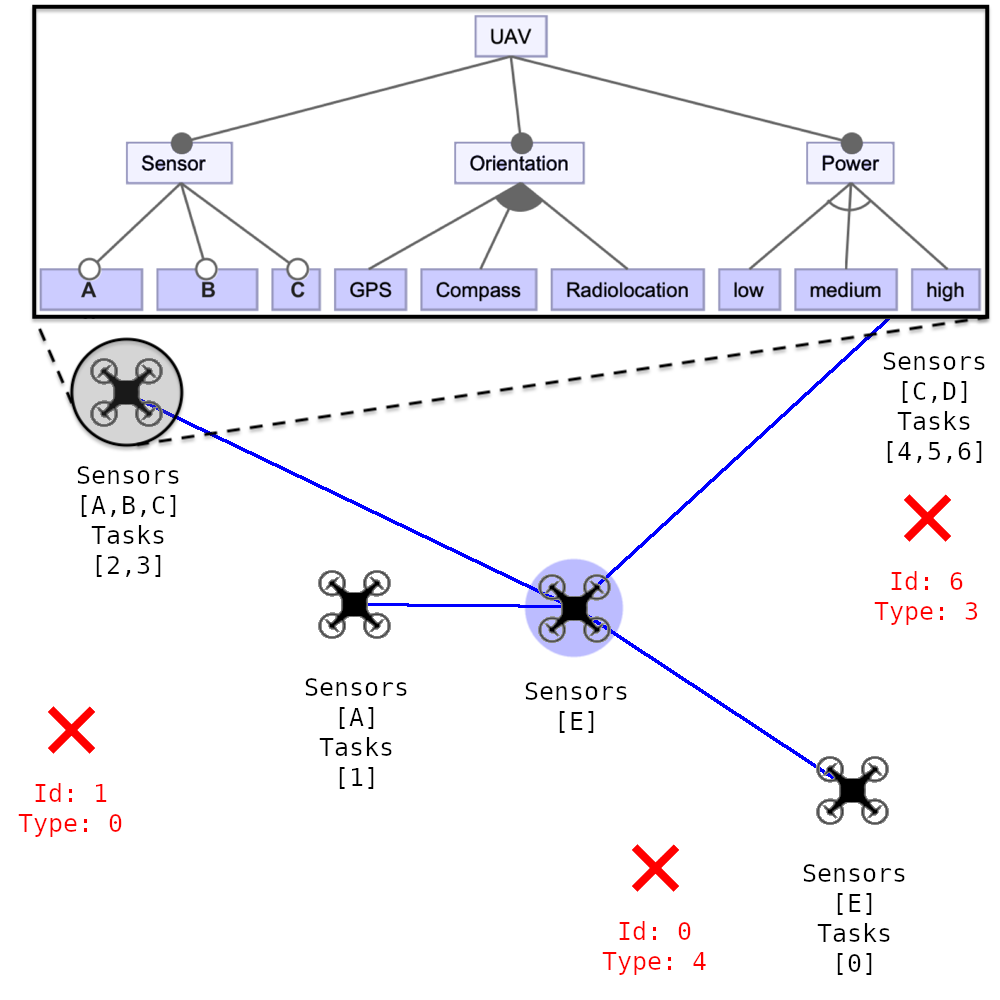
\includegraphics[width=0.95\linewidth]{img/scenario_01.png}
	    \caption{Feature Model showing UAV internal structure\label{fig:scene01}}
	\end{subfigure}
	\begin{subfigure}[t]{.45\textwidth}
	\centering
	    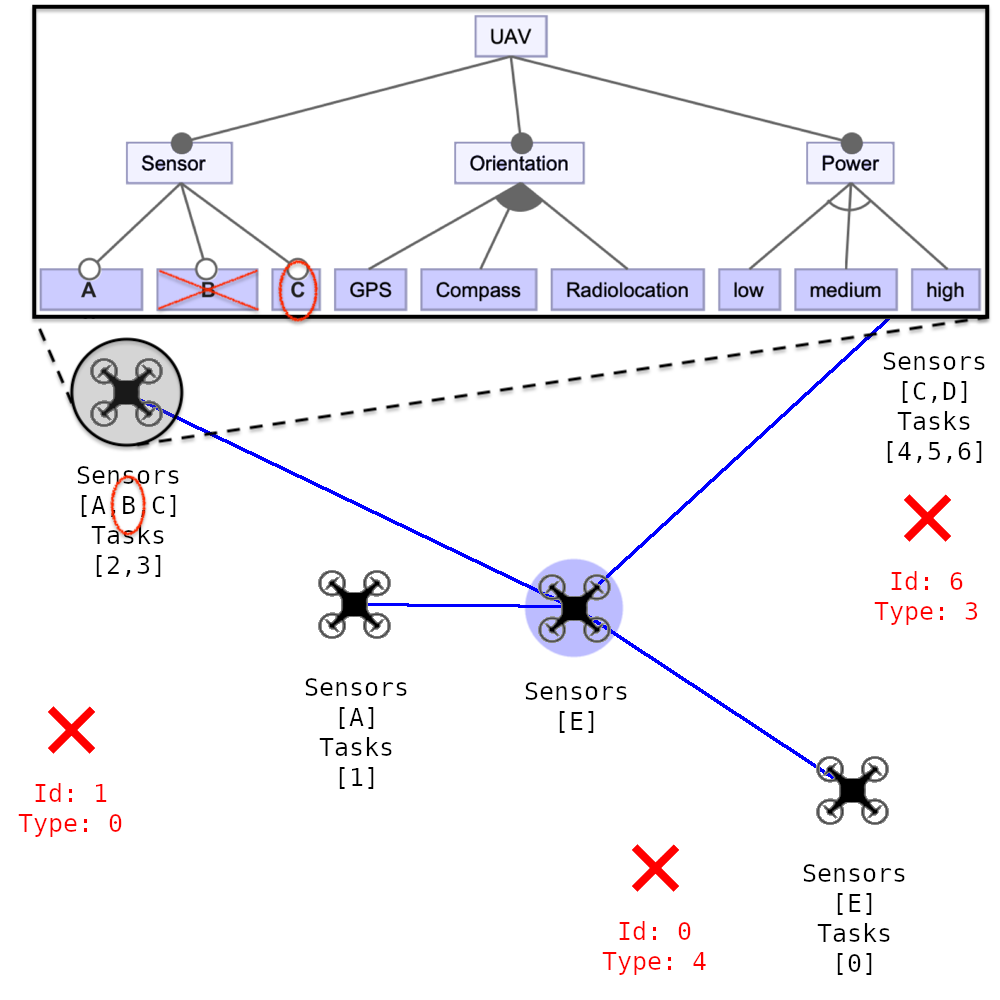
\includegraphics[width=0.95\linewidth]{img/scenario_02.png}
	    \caption{Feature activation to deal with context change\label{fig:scene02}}
	\end{subfigure}
	\caption{Member modeling using a Feature Model (partial view)indicating a reconfiguration performed by the TP, deactivating the feature related to sensor B and activating sensor C}
	\label{fig:TP_behavior}
\end{figure}

Based on this, a member $e$ is capable of executing a task $t$ when it reconfigures itself to adopt a configuration $c \in [\![FM]\!]$ such that this configuration makes the member capable of dealing with the task $t$.  This compatibility is known at the start and is denoted by $compatible(c, t)$. This configuration is characterized by sensors activated. There is a score, between 0 and 1, which indicates the compatibility level between each sensor $i$ onboard and the type of a task $j$, written as $Q_{ij}$ and so named quality. In summary, a member can receive a task $j$ when it has a sensor $i$ enabled whose $Q_{ij}$ meets the threshold, i.e., the acceptance level defined.  

%\begin{equation}
%    \label{eq:prop6}
%    compatible(e, t) \iff \exists c \in C_e \ \bullet compatible(c, t)
%\end{equation}

Figure~\ref{fig:ex_pg} defines \X{TP} behavior formally. Accordingly, upon mission start (guard $g_0$), TP has an initial configuration $c_0$, i.e., initial state defined by \X{members'} characteristics or even by the domain requirements, and an initial C2 strategy $w_0$ received through channel $ch2$ from $C2AM$ (location \textit{Idle}). An example of initial configuration is an energy safe mode, i.e., all sensors off, operated \X{to increase members' operating range}.

\begin{figure}[ht!]
    \centering
    \scalebox{.75}{

\tikzset{every picture/.style={line width=0.75pt}} %set default line width to 0.75pt        

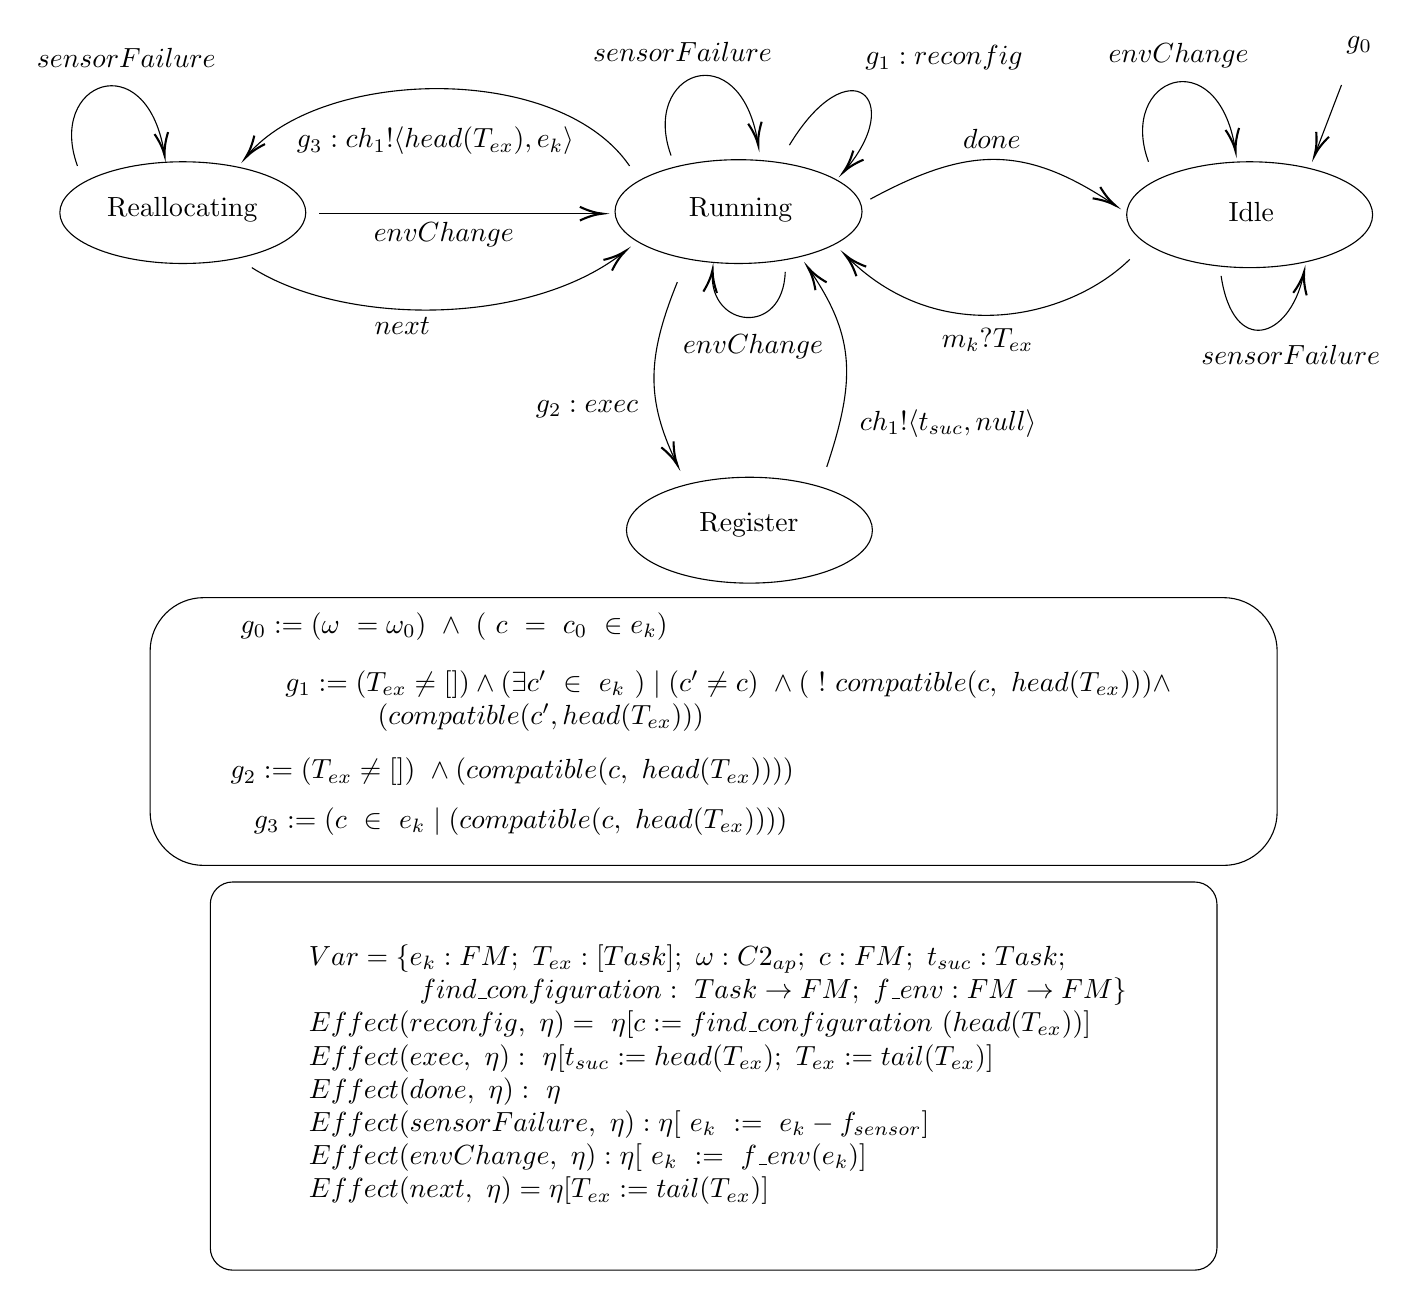
\begin{tikzpicture}[x=0.75pt,y=0.75pt,yscale=-1,xscale=1]
%uncomment if require: \path (0,620); %set diagram left start at 0, and has height of 620

%Curve Lines [id:da9480858267519683] 
\draw    (385.5,222) .. controls (399.29,180.63) and (399.5,159.63) .. (377.52,127.48) ;
\draw [shift={(376.5,126)}, rotate = 415.12] [color={rgb, 255:red, 0; green, 0; blue, 0 }  ][line width=0.75]    (10.93,-3.29) .. controls (6.95,-1.4) and (3.31,-0.3) .. (0,0) .. controls (3.31,0.3) and (6.95,1.4) .. (10.93,3.29)   ;
%Shape: Ellipse [id:dp6594609066072359] 
\draw   (283.5,99) .. controls (283.5,85.19) and (310.14,74) .. (343,74) .. controls (375.86,74) and (402.5,85.19) .. (402.5,99) .. controls (402.5,112.81) and (375.86,124) .. (343,124) .. controls (310.14,124) and (283.5,112.81) .. (283.5,99) -- cycle ;
%Shape: Ellipse [id:dp873836537729809] 
\draw   (530,100.5) .. controls (530,86.42) and (556.53,75) .. (589.25,75) .. controls (621.97,75) and (648.5,86.42) .. (648.5,100.5) .. controls (648.5,114.58) and (621.97,126) .. (589.25,126) .. controls (556.53,126) and (530,114.58) .. (530,100.5) -- cycle ;
%Curve Lines [id:da21020703050779688] 
\draw    (367.5,67) .. controls (396.21,19.48) and (423.94,44.49) .. (394.41,78.95) ;
\draw [shift={(393.5,80)}, rotate = 311.53] [color={rgb, 255:red, 0; green, 0; blue, 0 }  ][line width=0.75]    (10.93,-3.29) .. controls (6.95,-1.4) and (3.31,-0.3) .. (0,0) .. controls (3.31,0.3) and (6.95,1.4) .. (10.93,3.29)   ;
%Straight Lines [id:da37650774099478246] 
\draw    (633.5,38) -- (621.21,70.13) ;
\draw [shift={(620.5,72)}, rotate = 290.92] [color={rgb, 255:red, 0; green, 0; blue, 0 }  ][line width=0.75]    (10.93,-3.29) .. controls (6.95,-1.4) and (3.31,-0.3) .. (0,0) .. controls (3.31,0.3) and (6.95,1.4) .. (10.93,3.29)   ;
%Shape: Ellipse [id:dp02234558999259495] 
\draw   (16,99.5) .. controls (16,85.97) and (42.53,75) .. (75.25,75) .. controls (107.97,75) and (134.5,85.97) .. (134.5,99.5) .. controls (134.5,113.03) and (107.97,124) .. (75.25,124) .. controls (42.53,124) and (16,113.03) .. (16,99.5) -- cycle ;
%Curve Lines [id:da2517277021570281] 
\draw    (290.5,77) .. controls (255.85,26.51) and (141.81,29.93) .. (106.54,71.72) ;
\draw [shift={(105.5,73)}, rotate = 308.33000000000004] [color={rgb, 255:red, 0; green, 0; blue, 0 }  ][line width=0.75]    (10.93,-3.29) .. controls (6.95,-1.4) and (3.31,-0.3) .. (0,0) .. controls (3.31,0.3) and (6.95,1.4) .. (10.93,3.29)   ;
%Curve Lines [id:da851947022127026] 
\draw    (108.5,126) .. controls (152.06,153.72) and (240.7,154.98) .. (287.11,119.1) ;
\draw [shift={(288.5,118)}, rotate = 501.19] [color={rgb, 255:red, 0; green, 0; blue, 0 }  ][line width=0.75]    (10.93,-3.29) .. controls (6.95,-1.4) and (3.31,-0.3) .. (0,0) .. controls (3.31,0.3) and (6.95,1.4) .. (10.93,3.29)   ;
%Curve Lines [id:da05773774536505705] 
\draw    (531.5,122) .. controls (503.29,149.72) and (440.77,165.68) .. (395.86,121.36) ;
\draw [shift={(394.5,120)}, rotate = 405.63] [color={rgb, 255:red, 0; green, 0; blue, 0 }  ][line width=0.75]    (10.93,-3.29) .. controls (6.95,-1.4) and (3.31,-0.3) .. (0,0) .. controls (3.31,0.3) and (6.95,1.4) .. (10.93,3.29)   ;
%Rounded Rect [id:dp5913972444482631] 
\draw   (59.5,310.8) .. controls (59.5,296.55) and (71.05,285) .. (85.3,285) -- (576.7,285) .. controls (590.95,285) and (602.5,296.55) .. (602.5,310.8) -- (602.5,388.2) .. controls (602.5,402.45) and (590.95,414) .. (576.7,414) -- (85.3,414) .. controls (71.05,414) and (59.5,402.45) .. (59.5,388.2) -- cycle ;
%Rounded Rect [id:dp9206164489184118] 
\draw   (88.5,432.74) .. controls (88.5,426.81) and (93.31,422) .. (99.24,422) -- (562.76,422) .. controls (568.69,422) and (573.5,426.81) .. (573.5,432.74) -- (573.5,598.26) .. controls (573.5,604.19) and (568.69,609) .. (562.76,609) -- (99.24,609) .. controls (93.31,609) and (88.5,604.19) .. (88.5,598.26) -- cycle ;
%Curve Lines [id:da46585089178877326] 
\draw    (24.5,77) .. controls (9.65,36.41) and (57.53,18.36) .. (66.25,70.4) ;
\draw [shift={(66.5,72)}, rotate = 261.57] [color={rgb, 255:red, 0; green, 0; blue, 0 }  ][line width=0.75]    (10.93,-3.29) .. controls (6.95,-1.4) and (3.31,-0.3) .. (0,0) .. controls (3.31,0.3) and (6.95,1.4) .. (10.93,3.29)   ;
%Curve Lines [id:da24525569786800605] 
\draw    (575.5,130) .. controls (581.38,169.2) and (608.39,160.38) .. (615.11,129.89) ;
\draw [shift={(615.5,128)}, rotate = 460.62] [color={rgb, 255:red, 0; green, 0; blue, 0 }  ][line width=0.75]    (10.93,-3.29) .. controls (6.95,-1.4) and (3.31,-0.3) .. (0,0) .. controls (3.31,0.3) and (6.95,1.4) .. (10.93,3.29)   ;
%Curve Lines [id:da5617910694928671] 
\draw    (310.5,72) .. controls (295.65,31.41) and (343.53,13.36) .. (352.25,65.4) ;
\draw [shift={(352.5,67)}, rotate = 261.57] [color={rgb, 255:red, 0; green, 0; blue, 0 }  ][line width=0.75]    (10.93,-3.29) .. controls (6.95,-1.4) and (3.31,-0.3) .. (0,0) .. controls (3.31,0.3) and (6.95,1.4) .. (10.93,3.29)   ;
%Shape: Ellipse [id:dp893416141673501] 
\draw   (289,252.5) .. controls (289,238.42) and (315.53,227) .. (348.25,227) .. controls (380.97,227) and (407.5,238.42) .. (407.5,252.5) .. controls (407.5,266.58) and (380.97,278) .. (348.25,278) .. controls (315.53,278) and (289,266.58) .. (289,252.5) -- cycle ;
%Curve Lines [id:da2982425830385871] 
\draw    (313.5,133) .. controls (298.72,169.45) and (298.5,189.4) .. (312.84,219.61) ;
\draw [shift={(313.5,221)}, rotate = 244.18] [color={rgb, 255:red, 0; green, 0; blue, 0 }  ][line width=0.75]    (10.93,-3.29) .. controls (6.95,-1.4) and (3.31,-0.3) .. (0,0) .. controls (3.31,0.3) and (6.95,1.4) .. (10.93,3.29)   ;
%Curve Lines [id:da08998093824564413] 
\draw    (406.5,93) .. controls (454.02,67.26) and (480.96,67) .. (523.21,95.14) ;
\draw [shift={(524.5,96)}, rotate = 214] [color={rgb, 255:red, 0; green, 0; blue, 0 }  ][line width=0.75]    (10.93,-3.29) .. controls (6.95,-1.4) and (3.31,-0.3) .. (0,0) .. controls (3.31,0.3) and (6.95,1.4) .. (10.93,3.29)   ;
%Curve Lines [id:da7980176061132549] 
\draw    (365.5,128) .. controls (364.52,159.36) and (328.97,155.19) .. (330.37,128.65) ;
\draw [shift={(330.5,127)}, rotate = 456.12] [color={rgb, 255:red, 0; green, 0; blue, 0 }  ][line width=0.75]    (10.93,-3.29) .. controls (6.95,-1.4) and (3.31,-0.3) .. (0,0) .. controls (3.31,0.3) and (6.95,1.4) .. (10.93,3.29)   ;
%Curve Lines [id:da863076595467461] 
\draw    (540.5,75) .. controls (525.65,34.41) and (573.53,16.36) .. (582.25,68.4) ;
\draw [shift={(582.5,70)}, rotate = 261.57] [color={rgb, 255:red, 0; green, 0; blue, 0 }  ][line width=0.75]    (10.93,-3.29) .. controls (6.95,-1.4) and (3.31,-0.3) .. (0,0) .. controls (3.31,0.3) and (6.95,1.4) .. (10.93,3.29)   ;
%Straight Lines [id:da7258762513235244] 
\draw    (141,100) -- (275.5,100) ;
\draw [shift={(277.5,100)}, rotate = 180] [color={rgb, 255:red, 0; green, 0; blue, 0 }  ][line width=0.75]    (10.93,-3.29) .. controls (6.95,-1.4) and (3.31,-0.3) .. (0,0) .. controls (3.31,0.3) and (6.95,1.4) .. (10.93,3.29)   ;

% Text Node
\draw (344,98) node   [align=left] {Running};
% Text Node
\draw (590,99) node   [align=left] {Idle};
% Text Node
\draw (197,65) node    {$g_{3} :ch_{1} !\langle head( T_{ex}) ,e_{k} \rangle $};
% Text Node
\draw (463,161) node    {$m_{k} ?T_{ex}$};
% Text Node
\draw (75,98) node   [align=left] {Reallocating};
% Text Node
\draw (181,154) node    {$next$};
% Text Node
\draw (338,335) node    {$ \begin{array}{l}
g_{1} :=( T_{ex} \neq []) \land ( \exists c'\ \in \ \llbracket e_{k} \rrbracket \ ) \mid ( c'\neq c) \ \land ( \ !\ compatible( c,\ head( T_{ex}))) \land \\
\ \ \ \ \ \ \ \ \ \ ( compatible( c',head( T_{ex})))
\end{array}$};
% Text Node
\draw (442,25) node    {$g_{1} :reconfig$};
% Text Node
\draw (270,194) node    {$g_{2} :exec$};
% Text Node
\draw (234,369) node    {$g_{2} :=( T_{ex} \neq []) \ \land ( compatible( c,\ head( T_{ex}))))$};
% Text Node
\draw (232,472) node    {$ \begin{array}{l}
\end{array}$};
% Text Node
\draw (333,515) node    {$ \begin{array}{l}
Var=\{e_{k} :FM;\ T_{ex} :[ Task] ;\ \omega :C2_{ap} ;\ c:\llbracket FM\rrbracket ;\ t_{suc} :Task;\ \\
\ \ \ \ \ \ \ \ \ \ \ \ find\_configuration:\ Task\rightarrow \llbracket FM\rrbracket ;\ f\_env:FM\rightarrow FM\}\\
Effect( reconfig,\ \eta ) =\ \eta [ c:=find\_configuration\ ( head( T_{ex}))]\\
Effect( exec,\ \eta ) :\ \eta [ t_{suc} :=head( T_{ex}) ;\ T_{ex} :=tail( T_{ex})]\\
Effect( done,\ \eta ) :\ \eta \\
Effect( sensorFailure,\ \eta ) :\eta [ \ e_{k} \ :=\ e_{k} -f_{sensor}]\\
Effect( envChange,\ \eta ) :\eta [ \ e_{k} \ :=\ f\_env( e_{k})]\\
Effect( next,\ \eta ) =\eta [ T_{ex} :=tail( T_{ex})]
\end{array}$};
% Text Node
\draw (642,19) node    {$g_{0}$};
% Text Node
\draw (238,393) node    {$g_{3} :=( \nexists c\ \in \ \llbracket e_{k} \rrbracket \mid ( compatible( c,\ head( T_{ex}))))$};
% Text Node
\draw (206,299) node    {$g_{0} :=( \omega \ =\omega _{0}) \ \land \ ( \ c\ =\ c_{0} \ \in \llbracket e_{k} \rrbracket )$};
% Text Node
\draw (48,25) node    {$sensorFailure$};
% Text Node
\draw (609,168) node    {$sensorFailure$};
% Text Node
\draw (465,64) node    {$done$};
% Text Node
\draw (316,22) node    {$sensorFailure$};
% Text Node
\draw (348,250) node   [align=left] {Register};
% Text Node
\draw (444,201) node    {$ch_{1} !\langle t_{suc} ,null\rangle $};
% Text Node
\draw (201,110) node    {$envChange$};
% Text Node
\draw (350,164) node    {$envChange$};
% Text Node
\draw (555,24) node    {$envChange$};


\end{tikzpicture}}
    \caption{Program Graph defining the Task Performer $k$ (TP) role}
    \label{fig:ex_pg}
\end{figure}

After the initial guard condition $g_0$ is satisfied and the first location is reached, as shown in~Figure~\ref{fig:ex_pg}, TP can eventually be allocated tasks $T_{ex}$ that arrive over its dedicated asynchronous channel $m_k$ with the TA, at which point it will start addressing these in sequence (location \textit{Running}). If TP is able to execute the first allocated task (guard $g_2$), it indicates successful task execution with the $exec$ action, moving to location $Register$, and reports such task to the TA over the shared asynchronous channel $ch_1$, then moving back to location \textit{Running}. If the member still has a configuration capable of addressing the task (guard $g_1$), it will reconfigure to it. Otherwise (guard $g_3$), it will notify this problematic task to the TA (location \textit{Reallocating}) and continue execution (location \textit{Running}). 

Alternatively, the member may non-deterministically experience sensor failure (action $sensorFailure$), whose effect is described by removing configurations with the corresponding feature from the member's feature model, i.e., a self-reconfiguration that can be improved by a task reallocation. This action together with members loss (action $memberFailure$) composes changes in the self. In such a case, the tasks can be reallocated or a new C2 Approach can be operated to improve the system's awareness about the situation.

\X{
In summary, the member's implementation as DSPL provides the first level for dealing with context changes. Figure~\ref{fig:dspl_approach} shows the DSPL approach steps performed by the~\emph{Task Performer} PG. The \emph{FM}, which models such a DSPL, maps all sensors and other resources onboard in the UAV and we can activate or deactivate according to the features required and addressing all existing constraints between them. Such a mapping is oriented to maximize the quality and mission results.
}

\begin{figure}[ht]
    \centering
    \color{blue}
    \scalebox{.75}{

\tikzset{every picture/.style={line width=0.75pt}} %set default line width to 0.75pt        

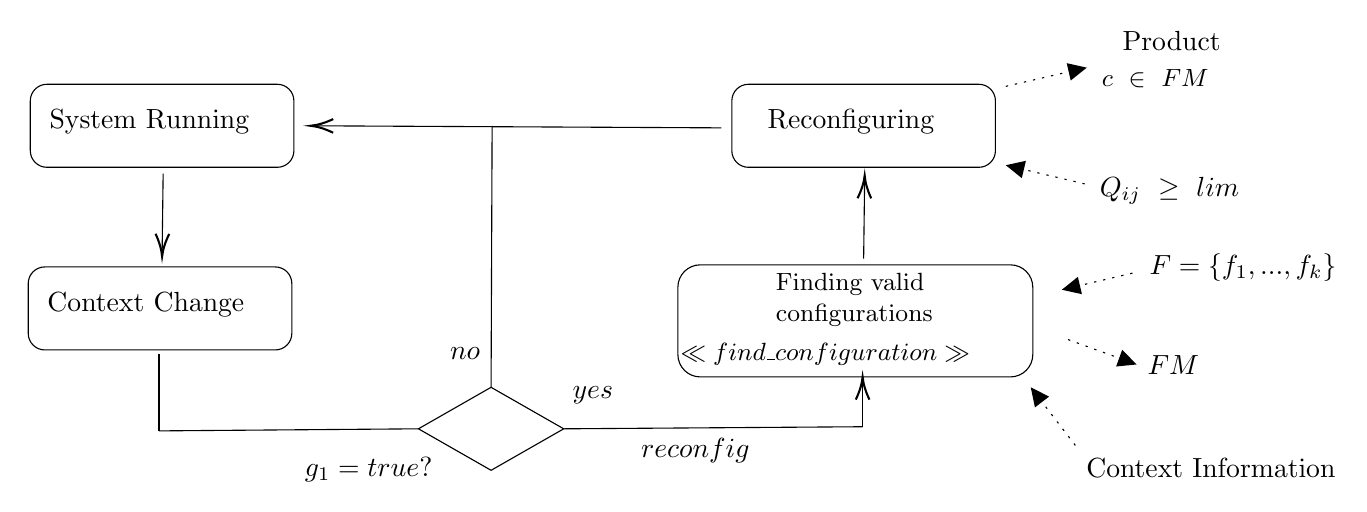
\begin{tikzpicture}[x=0.75pt,y=0.75pt,yscale=-1,xscale=1]
%uncomment if require: \path (0,244); %set diagram left start at 0, and has height of 244

%Rounded Rect [id:dp8066480632996035] 
\draw   (9,40) .. controls (9,35.58) and (12.58,32) .. (17,32) -- (128,32) .. controls (132.42,32) and (136,35.58) .. (136,40) -- (136,64) .. controls (136,68.42) and (132.42,72) .. (128,72) -- (17,72) .. controls (12.58,72) and (9,68.42) .. (9,64) -- cycle ;
%Rounded Rect [id:dp09986312472167136] 
\draw   (8,128) .. controls (8,123.58) and (11.58,120) .. (16,120) -- (127,120) .. controls (131.42,120) and (135,123.58) .. (135,128) -- (135,152) .. controls (135,156.42) and (131.42,160) .. (127,160) -- (16,160) .. controls (11.58,160) and (8,156.42) .. (8,152) -- cycle ;
%Rounded Rect [id:dp3203334247066908] 
\draw   (321,129.8) .. controls (321,123.84) and (325.84,119) .. (331.8,119) -- (481.2,119) .. controls (487.16,119) and (492,123.84) .. (492,129.8) -- (492,162.2) .. controls (492,168.16) and (487.16,173) .. (481.2,173) -- (331.8,173) .. controls (325.84,173) and (321,168.16) .. (321,162.2) -- cycle ;
%Straight Lines [id:da7215475210798592] 
\draw    (342,53) -- (146,52.01) ;
\draw [shift={(144,52)}, rotate = 0.29] [color={rgb, 255:red, 0; green, 0; blue, 0 }  ][line width=0.75]    (10.93,-3.29) .. controls (6.95,-1.4) and (3.31,-0.3) .. (0,0) .. controls (3.31,0.3) and (6.95,1.4) .. (10.93,3.29)   ;
%Straight Lines [id:da566488552820097] 
\draw    (73,75) -- (72.52,113) ;
\draw [shift={(72.5,115)}, rotate = 270.72] [color={rgb, 255:red, 0; green, 0; blue, 0 }  ][line width=0.75]    (10.93,-3.29) .. controls (6.95,-1.4) and (3.31,-0.3) .. (0,0) .. controls (3.31,0.3) and (6.95,1.4) .. (10.93,3.29)   ;
%Straight Lines [id:da03600720187770856] 
\draw  [dash pattern={on 0.84pt off 2.51pt}]  (509,155) -- (539.18,165.97) ;
\draw [shift={(542,167)}, rotate = 199.98] [fill={rgb, 255:red, 0; green, 0; blue, 0 }  ][line width=0.08]  [draw opacity=0] (8.93,-4.29) -- (0,0) -- (8.93,4.29) -- cycle    ;
%Rounded Rect [id:dp7101206593267378] 
\draw   (347,40) .. controls (347,35.58) and (350.58,32) .. (355,32) -- (466,32) .. controls (470.42,32) and (474,35.58) .. (474,40) -- (474,64) .. controls (474,68.42) and (470.42,72) .. (466,72) -- (355,72) .. controls (350.58,72) and (347,68.42) .. (347,64) -- cycle ;
%Straight Lines [id:da7286524767507477] 
\draw    (266,198) -- (410,197) ;
%Straight Lines [id:da695602580560019] 
\draw    (71,162) -- (71,199) ;
%Straight Lines [id:da47123812289807143] 
\draw    (410,175) -- (410,197) ;
\draw [shift={(410,173)}, rotate = 90] [color={rgb, 255:red, 0; green, 0; blue, 0 }  ][line width=0.75]    (10.93,-3.29) .. controls (6.95,-1.4) and (3.31,-0.3) .. (0,0) .. controls (3.31,0.3) and (6.95,1.4) .. (10.93,3.29)   ;
%Straight Lines [id:da7842612276994353] 
\draw  [dash pattern={on 0.84pt off 2.51pt}]  (517,80) -- (481.92,71.69) ;
\draw [shift={(479,71)}, rotate = 13.32] [fill={rgb, 255:red, 0; green, 0; blue, 0 }  ][line width=0.08]  [draw opacity=0] (8.93,-4.29) -- (0,0) -- (8.93,4.29) -- cycle    ;
%Straight Lines [id:da6842594623348534] 
\draw  [dash pattern={on 0.84pt off 2.51pt}]  (479,33) -- (515.08,24.67) ;
\draw [shift={(518,24)}, rotate = 167.01] [fill={rgb, 255:red, 0; green, 0; blue, 0 }  ][line width=0.08]  [draw opacity=0] (8.93,-4.29) -- (0,0) -- (8.93,4.29) -- cycle    ;
%Straight Lines [id:da2973367810568732] 
\draw    (410.98,78) -- (410.5,116) ;
\draw [shift={(411,76)}, rotate = 90.72] [color={rgb, 255:red, 0; green, 0; blue, 0 }  ][line width=0.75]    (10.93,-3.29) .. controls (6.95,-1.4) and (3.31,-0.3) .. (0,0) .. controls (3.31,0.3) and (6.95,1.4) .. (10.93,3.29)   ;
%Straight Lines [id:da9420001435559124] 
\draw  [dash pattern={on 0.84pt off 2.51pt}]  (540,123) -- (508.92,130.31) ;
\draw [shift={(506,131)}, rotate = 346.76] [fill={rgb, 255:red, 0; green, 0; blue, 0 }  ][line width=0.08]  [draw opacity=0] (8.93,-4.29) -- (0,0) -- (8.93,4.29) -- cycle    ;
%Flowchart: Decision [id:dp759598130534352] 
\draw   (231,178) -- (266,198) -- (231,218) -- (196,198) -- cycle ;
%Straight Lines [id:da367734053399414] 
\draw    (71,199) -- (196,198) ;
%Straight Lines [id:da5755851308332511] 
\draw    (231.5,52) -- (231,178) ;
%Straight Lines [id:da3242394337958049] 
\draw  [dash pattern={on 0.84pt off 2.51pt}]  (512.5,206) -- (492.83,180.38) ;
\draw [shift={(491,178)}, rotate = 52.48] [fill={rgb, 255:red, 0; green, 0; blue, 0 }  ][line width=0.08]  [draw opacity=0] (8.93,-4.29) -- (0,0) -- (8.93,4.29) -- cycle    ;

% Text Node
\draw (17,43) node [anchor=north west][inner sep=0.75pt]   [align=left] {System Running};
% Text Node
\draw (16,131) node [anchor=north west][inner sep=0.75pt]   [align=left] {Context Change};
% Text Node
\draw (367,122) node [anchor=north west][inner sep=0.75pt]  [font=\small] [align=left] {Finding valid\\configurations};
% Text Node
\draw (321,155.4) node [anchor=north west][inner sep=0.75pt]  [font=\small]  {$\ll find\_configuration\gg $};
% Text Node
\draw (546,161.4) node [anchor=north west][inner sep=0.75pt]    {$\llbracket FM\rrbracket $};
% Text Node
\draw (363,43) node [anchor=north west][inner sep=0.75pt]   [align=left] {Reconfiguring};
% Text Node
\draw (523,75.4) node [anchor=north west][inner sep=0.75pt]    {$Q_{ij} \ \geq \ lim$};
% Text Node
\draw (302,201.4) node [anchor=north west][inner sep=0.75pt]    {$reconfig$};
% Text Node
\draw (529,5) node [anchor=north west][inner sep=0.75pt]   [align=left] {\begin{minipage}[lt]{42.88pt}\setlength\topsep{0pt}
\begin{center}
Product
\end{center}

\end{minipage}};
% Text Node
\draw (547,112.4) node [anchor=north west][inner sep=0.75pt]    {$F=\{f_{1} ,...,f_{k}\}$};
% Text Node
\draw (524,23.4) node [anchor=north west][inner sep=0.75pt]  [font=\small]  {$c\ \in \ \llbracket FM\rrbracket $};
% Text Node
\draw (140,210.4) node [anchor=north west][inner sep=0.75pt]    {$g_{1} = true ?$};
% Text Node
\draw (269,176.4) node [anchor=north west][inner sep=0.75pt]    {$yes$};
% Text Node
\draw (210,157.4) node [anchor=north west][inner sep=0.75pt]    {$no$};
% Text Node
\draw (516.5,211) node [anchor=north west][inner sep=0.75pt]   [align=left] {Context Information};


\end{tikzpicture}}
    \caption{Task Performer actions related to the DSPL approach}
    \label{fig:dspl_approach}
\end{figure}

\X{
Any perturbation described in Section~\ref{sec:example} that becomes the member’s configuration incompatible with the circumstance, i.e., guard condition $g_1$ equals to true, activates the action~\emph{reconfig}, that provides all mission's required feature activation. It requires an adjustment to perform the next task or to continue the current execution. Algorithm~\ref{algo:reconfig_algo} describes the function~\emph{find\_configuration} that implements this action, which starts operating on the set of features $F$ to analyze their current status, and to generate an updated set of feature models $\llbracket FM \rrbracket$ compatible with the new circumstance (line~\ref{line:get_fm}). In addition, this reconfiguration may use information came from the context, e.g., tasks allocation between other members in the team. 
}

\begin{algorithm}[h!t]
    \SetAlCapNameFnt{\small}
    \SetAlCapFnt{\small\color{blue}}
	\caption{The function $find\_configuration$ that implements the the $reconfig$ action to deal with new circumstance}
	\label{algo:reconfig_algo}
	
	\color{blue}
	\SetAlgoLined
	\DontPrintSemicolon
	\SetKwBlock{Loop}{loop}{end loop}
	\SetKwFor{ForAll}{for all}{do}{end for}
	
	%\SetAlgoNlRelativeSize{-3}
	\SetNlSty{text}{}{:}
	\SetNlSkip{0.3em}

    i = current or next task\;
    quality = 0\;
    selected\_sensor = 0\;
    $\llbracket FM \rrbracket$ = valid configurations based on $F$\;\label{line:get_fm}
    \ForAll{ onboard sensor j }{\label{line:select_sensor_begin}
     $Q_{ij}$ = calculate quality to sensor $j$ be used in task $i$\;\label{line:calculate_quality}
     \If{($Q_{ij} \geq$ threshold)  $\land$  ($Q_{ij} >$ quality)}{quality = $Q_{ij}$\;\label{line:update_quality}
     selected\_sensor = j\;\label{line:select_sensor_end}}
    }
    select $c \in \llbracket FM \rrbracket \mid (number feature_{selected\_sensor} \in c$)\;\label{line:select_c}
    \ForAll{feature $f \in F$}{\label{line:select_f_begin}
    \If{$f \in c$}{activate $f$}
    \Else{deactivate $f$}\label{line:select_f_end}
    }
\end{algorithm}

\X{
Next, we perform a quality comparison of the task $i$ and each sensor $j$, according to their compatibility. The reconfiguration itself selects the best configuration $c$ to satisfy required quality parameter, i.e., \emph{threshold} (lines~\ref{line:select_sensor_begin} to~\ref{line:select_sensor_end}). After this analysis, we select the most suitable configuration $c$ that contains only the required sensor $j$ activated(line~\ref{line:select_c}). In such a case, all other sensor are disabled (lines~\ref{line:select_f_begin} to~\ref{line:select_f_end}).
}




\subsubsection{Task Allocator}

In contrast to role TP, which focuses on task execution and member reconfiguration, TA defines coordination behavior among members, establishing task allocation responsibilities, as shown formally in Figure~\ref{fig:ta_pg}. \X{The members with such a role perform the tasks allocation according to quality levels. In addition, they reallocate tasks because of context changes. Figure~\ref{fig:TA_behavior} shows a task reallocation because of sensor issue, looking for keeping mission's quality level.}

\begin{figure}[ht!]
    \centering
    \scalebox{.75}{

\tikzset{every picture/.style={line width=0.75pt}} %set default line width to 0.75pt        

\begin{tikzpicture}[x=0.75pt,y=0.75pt,yscale=-1,xscale=1]
%uncomment if require: \path (0,763); %set diagram left start at 0, and has height of 763

%Curve Lines [id:da9480858267519683] 
\draw    (201.5,185) .. controls (235.16,142.43) and (344.78,139.06) .. (377.05,182.66) ;
\draw [shift={(378,184)}, rotate = 235.44] [color={rgb, 255:red, 0; green, 0; blue, 0 }  ][line width=0.75]    (10.93,-3.29) .. controls (6.95,-1.4) and (3.31,-0.3) .. (0,0) .. controls (3.31,0.3) and (6.95,1.4) .. (10.93,3.29)   ;
%Shape: Ellipse [id:dp6594609066072359] 
\draw   (91.5,212) .. controls (91.5,198.19) and (118.14,187) .. (151,187) .. controls (183.86,187) and (210.5,198.19) .. (210.5,212) .. controls (210.5,225.81) and (183.86,237) .. (151,237) .. controls (118.14,237) and (91.5,225.81) .. (91.5,212) -- cycle ;
%Shape: Ellipse [id:dp873836537729809] 
\draw   (368,205.5) .. controls (368,191.42) and (394.53,180) .. (427.25,180) .. controls (459.97,180) and (486.5,191.42) .. (486.5,205.5) .. controls (486.5,219.58) and (459.97,231) .. (427.25,231) .. controls (394.53,231) and (368,219.58) .. (368,205.5) -- cycle ;
%Curve Lines [id:da14662580418826565] 
\draw    (485.5,428) .. controls (538.96,423.05) and (565.96,389.68) .. (574.25,345.35) ;
\draw [shift={(574.5,344)}, rotate = 460.08] [color={rgb, 255:red, 0; green, 0; blue, 0 }  ][line width=0.75]    (10.93,-3.29) .. controls (6.95,-1.4) and (3.31,-0.3) .. (0,0) .. controls (3.31,0.3) and (6.95,1.4) .. (10.93,3.29)   ;
%Straight Lines [id:da37650774099478246] 
\draw    (203.5,18) -- (234.11,28.36) ;
\draw [shift={(236,29)}, rotate = 198.7] [color={rgb, 255:red, 0; green, 0; blue, 0 }  ][line width=0.75]    (10.93,-3.29) .. controls (6.95,-1.4) and (3.31,-0.3) .. (0,0) .. controls (3.31,0.3) and (6.95,1.4) .. (10.93,3.29)   ;
%Shape: Ellipse [id:dp8139093405894636] 
\draw   (92,423) .. controls (92,409.19) and (118.53,398) .. (151.25,398) .. controls (183.97,398) and (210.5,409.19) .. (210.5,423) .. controls (210.5,436.81) and (183.97,448) .. (151.25,448) .. controls (118.53,448) and (92,436.81) .. (92,423) -- cycle ;
%Shape: Ellipse [id:dp08678607998247811] 
\draw   (362,422) .. controls (362,408.19) and (388.53,397) .. (421.25,397) .. controls (453.97,397) and (480.5,408.19) .. (480.5,422) .. controls (480.5,435.81) and (453.97,447) .. (421.25,447) .. controls (388.53,447) and (362,435.81) .. (362,422) -- cycle ;
%Shape: Ellipse [id:dp07482494496489733] 
\draw   (241,32) .. controls (241,18.75) and (267.53,8) .. (300.25,8) .. controls (332.97,8) and (359.5,18.75) .. (359.5,32) .. controls (359.5,45.25) and (332.97,56) .. (300.25,56) .. controls (267.53,56) and (241,45.25) .. (241,32) -- cycle ;
%Curve Lines [id:da6759956440889884] 
\draw    (94.5,230) .. controls (71.84,275.31) and (79.27,368.16) .. (97.65,405.34) ;
\draw [shift={(98.5,407)}, rotate = 242.18] [color={rgb, 255:red, 0; green, 0; blue, 0 }  ][line width=0.75]    (10.93,-3.29) .. controls (6.95,-1.4) and (3.31,-0.3) .. (0,0) .. controls (3.31,0.3) and (6.95,1.4) .. (10.93,3.29)   ;
%Curve Lines [id:da9572857730465772] 
\draw    (205.22,232.76) .. controls (231.54,272.31) and (232.61,380.42) .. (207,408) ;
\draw [shift={(204,231)}, rotate = 54.11] [color={rgb, 255:red, 0; green, 0; blue, 0 }  ][line width=0.75]    (10.93,-3.29) .. controls (6.95,-1.4) and (3.31,-0.3) .. (0,0) .. controls (3.31,0.3) and (6.95,1.4) .. (10.93,3.29)   ;
%Curve Lines [id:da9385545433271328] 
\draw    (488.5,319) .. controls (450.88,330.88) and (434.82,343.74) .. (428.68,389.6) ;
\draw [shift={(428.5,391)}, rotate = 277.28] [color={rgb, 255:red, 0; green, 0; blue, 0 }  ][line width=0.75]    (10.93,-3.29) .. controls (6.95,-1.4) and (3.31,-0.3) .. (0,0) .. controls (3.31,0.3) and (6.95,1.4) .. (10.93,3.29)   ;
%Curve Lines [id:da13526468384837043] 
\draw    (411.5,177) .. controls (397.78,123.1) and (372.54,74) .. (348.94,54.18) ;
\draw [shift={(347.5,53)}, rotate = 398.37] [color={rgb, 255:red, 0; green, 0; blue, 0 }  ][line width=0.75]    (10.93,-3.29) .. controls (6.95,-1.4) and (3.31,-0.3) .. (0,0) .. controls (3.31,0.3) and (6.95,1.4) .. (10.93,3.29)   ;
%Curve Lines [id:da7876400787103589] 
\draw    (238.5,49) .. controls (209.79,67.81) and (184.02,110.14) .. (172.83,174.06) ;
\draw [shift={(172.5,176)}, rotate = 279.61] [color={rgb, 255:red, 0; green, 0; blue, 0 }  ][line width=0.75]    (10.93,-3.29) .. controls (6.95,-1.4) and (3.31,-0.3) .. (0,0) .. controls (3.31,0.3) and (6.95,1.4) .. (10.93,3.29)   ;
%Shape: Ellipse [id:dp538933115831977] 
\draw   (495,314) .. controls (495,300.19) and (521.3,289) .. (553.75,289) .. controls (586.2,289) and (612.5,300.19) .. (612.5,314) .. controls (612.5,327.81) and (586.2,339) .. (553.75,339) .. controls (521.3,339) and (495,327.81) .. (495,314) -- cycle ;
%Curve Lines [id:da663291454681702] 
\draw    (489.5,209) .. controls (537.52,209) and (553.85,249.34) .. (555.42,282.01) ;
\draw [shift={(555.5,284)}, rotate = 268.26] [color={rgb, 255:red, 0; green, 0; blue, 0 }  ][line width=0.75]    (10.93,-3.29) .. controls (6.95,-1.4) and (3.31,-0.3) .. (0,0) .. controls (3.31,0.3) and (6.95,1.4) .. (10.93,3.29)   ;
%Curve Lines [id:da17641910717404863] 
\draw    (384.5,395) .. controls (365.69,327.68) and (270.43,245.66) .. (217.1,220.74) ;
\draw [shift={(215.5,220)}, rotate = 384.36] [color={rgb, 255:red, 0; green, 0; blue, 0 }  ][line width=0.75]    (10.93,-3.29) .. controls (6.95,-1.4) and (3.31,-0.3) .. (0,0) .. controls (3.31,0.3) and (6.95,1.4) .. (10.93,3.29)   ;
%Rounded Rect [id:dp2887172897272543] 
\draw   (20,546.88) .. controls (20,540.32) and (25.32,535) .. (31.88,535) -- (598.12,535) .. controls (604.68,535) and (610,540.32) .. (610,546.88) -- (610,738.12) .. controls (610,744.68) and (604.68,750) .. (598.12,750) -- (31.88,750) .. controls (25.32,750) and (20,744.68) .. (20,738.12) -- cycle ;
%Rounded Rect [id:dp07131134126212679] 
\draw   (19,477.2) .. controls (19,471.01) and (24.01,466) .. (30.2,466) -- (596.8,466) .. controls (602.99,466) and (608,471.01) .. (608,477.2) -- (608,510.8) .. controls (608,516.99) and (602.99,522) .. (596.8,522) -- (30.2,522) .. controls (24.01,522) and (19,516.99) .. (19,510.8) -- cycle ;
%Curve Lines [id:da580151899278355] 
\draw    (99,193) .. controls (71.91,170.34) and (103.04,144.78) .. (124.05,182.24) ;
\draw [shift={(125,184)}, rotate = 242.3] [color={rgb, 255:red, 0; green, 0; blue, 0 }  ][line width=0.75]    (10.93,-3.29) .. controls (6.95,-1.4) and (3.31,-0.3) .. (0,0) .. controls (3.31,0.3) and (6.95,1.4) .. (10.93,3.29)   ;

% Text Node
\draw (151,210) node   [align=left] {Ready};
% Text Node
\draw (428,204) node   [align=left] {Allocating};
% Text Node
\draw (294,171) node    {$T'\ \neq [] :allocate$};
% Text Node
\draw (153,422) node   [align=left] {Updating};
% Text Node
\draw (555,313) node   [align=left] {Notifying};
% Text Node
\draw (301,31) node   [align=left] {Waiting};
% Text Node
\draw (42,323) node    {$ch_{1} ?\langle t,e' \rangle $};
% Text Node
\draw (192,307) node    {$update$};
% Text Node
\draw (458,88) node    {$alloc=[] :ch_{3} !\langle T',E'\rangle $};
% Text Node
\draw (146,83) node    {$ch_{2} ?\langle T',E',\omega \rangle $};
% Text Node
\draw (423,420) node   [align=left] {Binding};
% Text Node
\draw (570,430) node    {$alloc\neq [] :bind$};
% Text Node
\draw (416,331) node    {$m_{k\ } !\ T'_{k}$};
% Text Node
\draw (567,199) node    {$alloc\neq [] :bind$};
% Text Node
\draw (362,270) node    {$alloc=[] :done$};
% Text Node
\draw (317,641) node    {$ \begin{array}{l}
Var=\{\ alloc:[ \langle \ \mathbb{N} ,[ Task] \ \rangle ] ;\ f\_alloc:([ Task] ,[ FM] ,C2_{ap}) \ \rightarrow [ \langle \ \mathbb{N} ,[ Task] \ \rangle ] ;\ \\
\ \ \ \ \ \ \ \ \ \ \ \ teamStatus:[ FM] \ \rightarrow \ \langle [ Task] ,[ FM] \rangle ;\ T':[ Task] ;\ T_{success} :[ Task] ;\ \\
\ \ \ \ \ \ \ \ \ \ \ \ E':[ FM] ;\ t:Task;\ e' :FM;\ \omega :C2_{ap} ;\ T_{add} :[ Task] \ \}\\
Effect( allocate,\ \eta ) =\ \eta [ alloc:=\ f\_alloc( T',\ E',\ \omega )]\\
Effect( bind,\ \eta ) =\ \eta [ \ \langle k,T'_{k} \rangle :=head( alloc) ;\ alloc:=tail( alloc) \ ]\\
Effect( update,\ \eta ) =\begin{cases}
\eta [ \ T_{success} :=T_{success} \ ++\ [ t] \ ] & \ \ \ \ if\ ( e'=null)\\
\eta [ \ T':=T'++\ [ t] \ ;\ E':=E'( e/e'_{\ })] & \ \ \ \ otherwise
\end{cases} \ \\
Effect( done,\eta ) =\eta [ \ T':=[] \ ]\\
Effect( memberFailure,\eta ) =\eta [ \ \langle T',E'\rangle :=teamStatus( E') \ ]
\end{array}$};
% Text Node
\draw (190,12) node    {$g_{0}$};
% Text Node
\draw (313.76,495) node    {$ \begin{array}{l}
g_{0} :=( T'=[]) \ \land ( f\_alloc\ =\ f_{x}([ t_{1} ,\ ...,t_{n}] \ p_{1} ,\ [ e_{1} ,...,e_{n}] \ p_{2} ,\ C2_{ap} \ p_{3})) \ \\
\ \ \ \ \ \ \ \ \ \land ( T_{success} =[]) \ \land \ ( \omega =\omega _{0})
\end{array}$};
% Text Node
\draw (68,148) node    {$memberFailure$};


\end{tikzpicture}}
    \caption{Program Graph defining the Task Allocator (TA) role}
    \label{fig:ta_pg}
\end{figure}


When the mission starts, TA is in the \textit{Waiting} location, staying there until it receives mission tasks $T'$ and members information $E'$ from the C2AM over the synchronous channel $ch_2$, then moving to location $Ready$. TA then performs task allocation (action $allocate$),  notifies each member $k$ (locations \textit{Notifying} and \textit{Binding}) of its assigned task $T'_k$ via an specific asynchronous channel $m_k$, returning to the \textit{Ready} location. Eventually, TA will be notified, over a shared asynchronous channel $ch_1$, of successfully completed tasks by the members and of failed tasks, in which case it will perform a new task allocation. In case of members' failure (action $memberFailure$), the TA tries to reallocate tasks previously allocated to those members. If unsuccessful, the TA reports such tasks along with members' status to the C2AM over the synchronous channel $ch_3$. 

\begin{figure}[!htbp]
	\centering
	\begin{subfigure}[t]{.45\textwidth}
	\centering
	    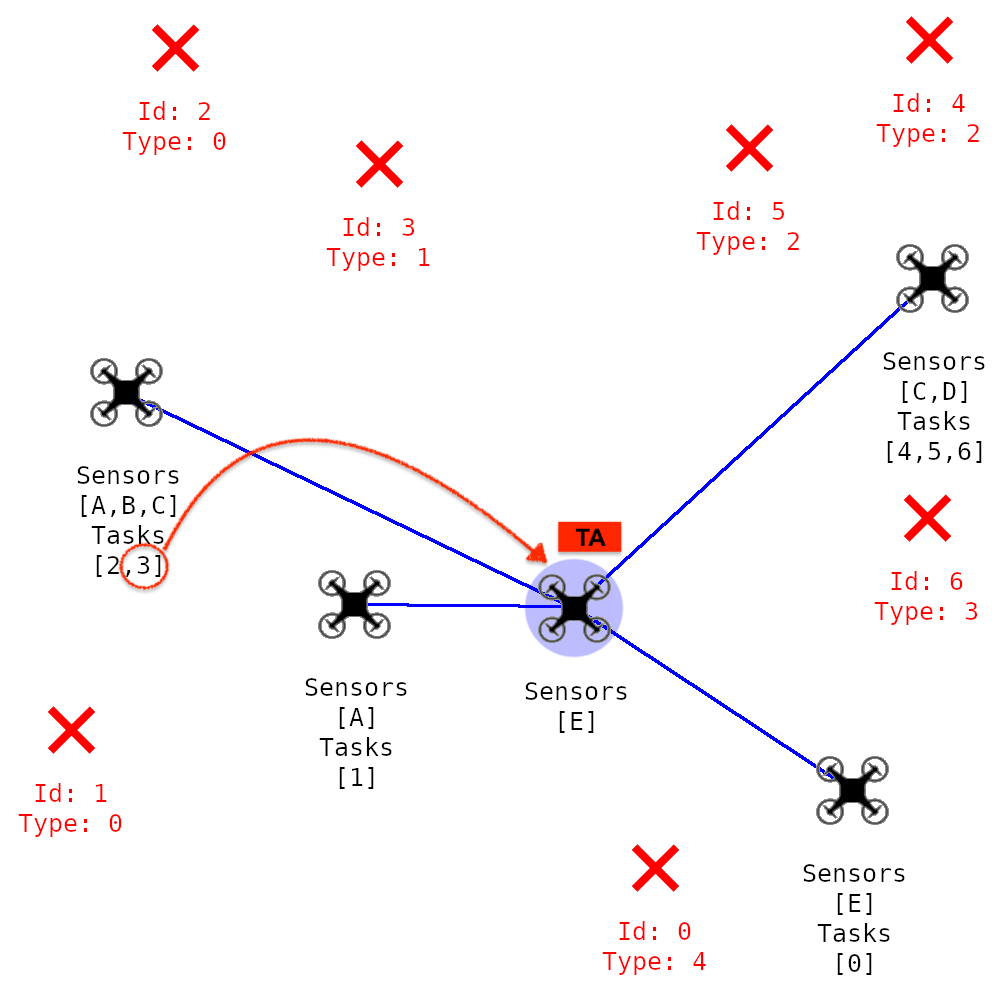
\includegraphics[width=0.95\linewidth]{img/scenario_03.png}
	    \caption{Member sends back a task not executable due to internal issues\label{fig:scene03}}
	\end{subfigure}
	\begin{subfigure}[t]{.45\textwidth}
	\centering
	    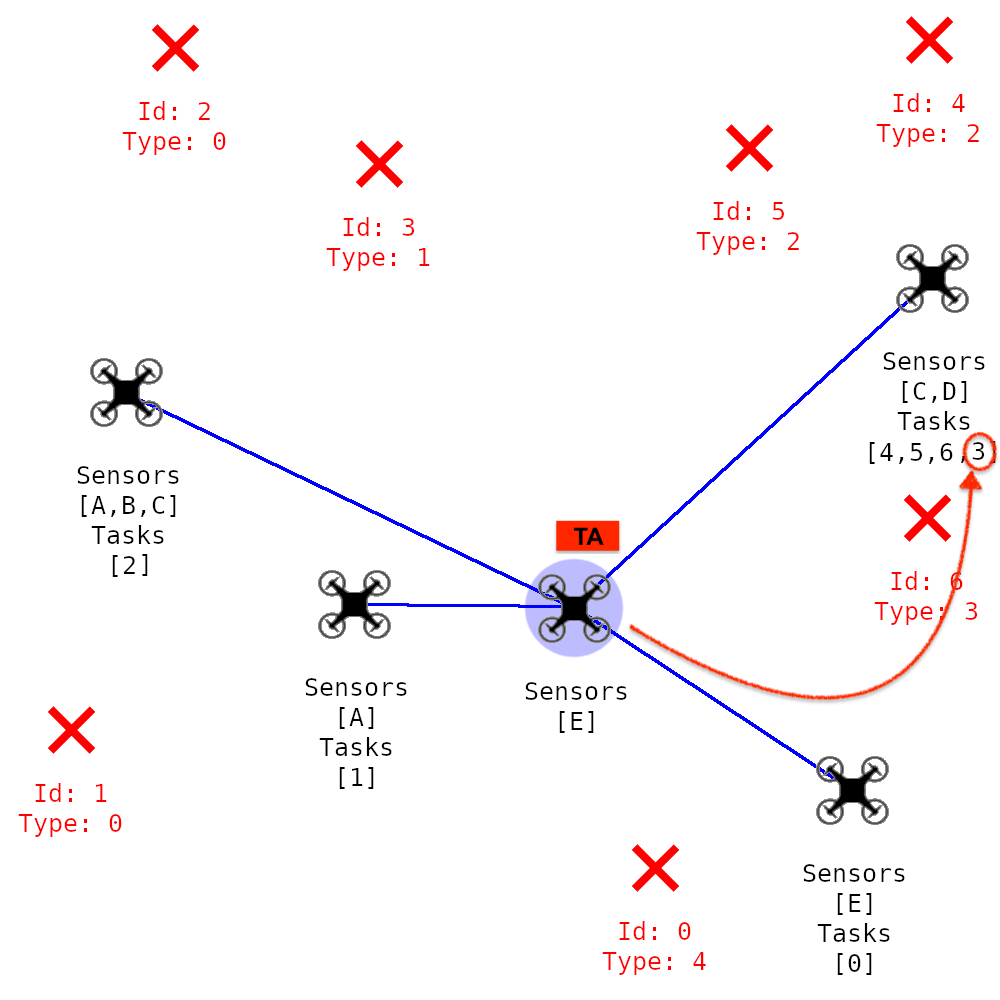
\includegraphics[width=0.95\linewidth]{img/scenario_04.png}
	    \caption{TA finds another member with a suitable sensor to send the task received \label{fig:scene04}}
	\end{subfigure}
	\caption{A task reallocation (task \#3) performed by a member with Task Allocator role, based on its compatibility's degree with the members' onboard sensors}
	\label{fig:TA_behavior}
\end{figure}


%Furthermore, the PG can absorb new tasks ($T_{add}$) added to the mission through the action $addTasks$, causing the mission update, represented by $T'++T_{add}$. 




\subsubsection{C2 Approach Manager}

At the coarsest-grained level of coordination, C2AM specifies a C2 approach change protocol, as defined formally in Figure~\ref{fig:c2a_pg}. C2AM starts operation by receiving mission tasks, member information, and initial C2 approach from the C2CS call ($g_0$ at location \textit{Notifying}), i.e., mission startup. From this initial location, it goes to the location \textit{Operating} with the initial C2 approach $\omega_0$ and sends the set of tasks $T$, the team $E$ and the $\omega_0$ over the synchronous channel $ch_2$. The C2AM remains in the $Operating$ location until eventually receiving, from TA, the pair formed by the set of unallocated tasks and the updated team members. Such information comes over the synchronous channel $ch_3$ and takes C2AM to location \textit{Maneuvering}.

The tasks received and the last information about the members' status are analyzed with the action $update$. \X{The function~\emph{find\_maneuver} takes the next C2 approach with higher awareness (cf. Section~\ref{sec:background}), according to~\citet{nato01}, and it checks if this choice is suitable for dealing with the context. In case this function finds a C2 Approach to be applied in order to perform the tasks with the available team, it is defined and C2AM sends mission tasks, members' information and C2 Approach selected to the TA over the synchronous channel $ch_2$, then moving to the location \emph{Operating}.} Otherwise, those tasks are registered as failed ($T_{fail}$) and the TA is notified with an empty set of tasks. The C2AM then goes to location \emph{Operating} passing through \emph{Notifying} and adopts a domain defined C2 Approach $w_f$ (cf. Section~\ref{ssec:background_c2}). \X{The results of these steps is shown in Figure~\ref{fig:TeamExecutionAfterManuever}.}

\begin{figure}[!ht]
    \centering
    \scalebox{.65}{

\tikzset{every picture/.style={line width=0.75pt}} %set default line width to 0.75pt        

\begin{tikzpicture}[x=0.75pt,y=0.75pt,yscale=-1,xscale=1]
%uncomment if require: \path (0,370); %set diagram left start at 0, and has height of 370

%Curve Lines [id:da9480858267519683] 
\draw    (200.5,59) .. controls (307.46,9.25) and (417.89,17.91) .. (502.72,60.36) ;
\draw [shift={(504,61)}, rotate = 206.82999999999998] [color={rgb, 255:red, 0; green, 0; blue, 0 }  ][line width=0.75]    (10.93,-3.29) .. controls (6.95,-1.4) and (3.31,-0.3) .. (0,0) .. controls (3.31,0.3) and (6.95,1.4) .. (10.93,3.29)   ;
%Shape: Ellipse [id:dp6594609066072359] 
\draw   (81.5,75) .. controls (81.5,61.19) and (108.14,50) .. (141,50) .. controls (173.86,50) and (200.5,61.19) .. (200.5,75) .. controls (200.5,88.81) and (173.86,100) .. (141,100) .. controls (108.14,100) and (81.5,88.81) .. (81.5,75) -- cycle ;
%Shape: Ellipse [id:dp873836537729809] 
\draw   (506,76.5) .. controls (506,62.42) and (532.53,51) .. (565.25,51) .. controls (597.97,51) and (624.5,62.42) .. (624.5,76.5) .. controls (624.5,90.58) and (597.97,102) .. (565.25,102) .. controls (532.53,102) and (506,90.58) .. (506,76.5) -- cycle ;
%Straight Lines [id:da37650774099478246] 
\draw    (334,149) -- (347.58,122.78) ;
\draw [shift={(348.5,121)}, rotate = 477.38] [color={rgb, 255:red, 0; green, 0; blue, 0 }  ][line width=0.75]    (10.93,-3.29) .. controls (6.95,-1.4) and (3.31,-0.3) .. (0,0) .. controls (3.31,0.3) and (6.95,1.4) .. (10.93,3.29)   ;
%Rounded Rect [id:dp20897962983691354] 
\draw   (118.5,186.6) .. controls (118.5,179.64) and (124.14,174) .. (131.1,174) -- (613.9,174) .. controls (620.86,174) and (626.5,179.64) .. (626.5,186.6) -- (626.5,224.4) .. controls (626.5,231.36) and (620.86,237) .. (613.9,237) -- (131.1,237) .. controls (124.14,237) and (118.5,231.36) .. (118.5,224.4) -- cycle ;
%Rounded Rect [id:dp6489541210438411] 
\draw   (7,266.4) .. controls (7,253.48) and (17.48,243) .. (30.4,243) -- (737.6,243) .. controls (750.52,243) and (761,253.48) .. (761,266.4) -- (761,336.6) .. controls (761,349.52) and (750.52,360) .. (737.6,360) -- (30.4,360) .. controls (17.48,360) and (7,349.52) .. (7,336.6) -- cycle ;
%Shape: Ellipse [id:dp35747792046006877] 
\draw   (297,90.5) .. controls (297,76.42) and (323.53,65) .. (356.25,65) .. controls (388.97,65) and (415.5,76.42) .. (415.5,90.5) .. controls (415.5,104.58) and (388.97,116) .. (356.25,116) .. controls (323.53,116) and (297,104.58) .. (297,90.5) -- cycle ;
%Curve Lines [id:da035475864760055154] 
\draw    (424.21,92.88) .. controls (460.08,106.96) and (486.38,105.74) .. (505,93) ;
\draw [shift={(422,92)}, rotate = 22.07] [color={rgb, 255:red, 0; green, 0; blue, 0 }  ][line width=0.75]    (10.93,-3.29) .. controls (6.95,-1.4) and (3.31,-0.3) .. (0,0) .. controls (3.31,0.3) and (6.95,1.4) .. (10.93,3.29)   ;
%Curve Lines [id:da19760874620395663] 
\draw    (202.22,95.88) .. controls (238.39,109.99) and (272.38,109.74) .. (291,97) ;
\draw [shift={(200,95)}, rotate = 22.07] [color={rgb, 255:red, 0; green, 0; blue, 0 }  ][line width=0.75]    (10.93,-3.29) .. controls (6.95,-1.4) and (3.31,-0.3) .. (0,0) .. controls (3.31,0.3) and (6.95,1.4) .. (10.93,3.29)   ;

% Text Node
\draw (139,74) node   [align=left] {Operating};
% Text Node
\draw (566,76) node   [align=left] {Maneuvering};
% Text Node
\draw (359,11) node    {$ch_{3} \ ?\langle T,E\rangle $};
% Text Node
\draw (349,147) node    {$g_{0}$};
% Text Node
\draw (469,115) node    {$update$};
% Text Node
\draw (374,203) node    {$ \begin{array}{l}
g_{0} =( \omega =\omega _{0}) \land ( find\_maneuver=f_{1}( C2_{ap} ,[ e_{1} ,...,e_{n}] ,[ t_{1} ,...,t_{n}])\\
\ \ \ \ \ \ \ \ \land ( E=\{e_{1} ,e_{2} ,...,e_{n}\}) \land ( T_{fail} =[]) \land ( T=[ t_{1} ,t_{2} ,...,t_{f}])
\end{array}$};
% Text Node
\draw (385,300) node    {$ \begin{array}{l}
Var=\{find\_maneuver:( C2_{ap} ,\ [ FM] ,\ [ Task])\rightarrow C2_{ap} ;\ T_{fail} :[ Task] ;\ \omega :C2_{ap} ;\ T:[ Task] ;\ E:[ FM] ;\\
\ \ \ \ \ \ \ \ \ \ \ \ \ \omega _{f} :C2_{ap} \ \}\\
Effect( update,\ \eta ) =\begin{cases}
\eta [ T_{fail} :=T_{fail} ++T;\ T:=[] ;\ \omega :=\omega _{f} \ ] & \ \ \ \ if\ ( find\_maneuver( \omega ,E,T) =NULL)\\
\eta [ \ \omega :=\ find\_maneuver( \omega ,\ E,\ T)] & \ \ \ \ otherwise
\end{cases}
\end{array}$};
% Text Node
\draw (246,120) node    {$ch_{2} !\langle T,E,\omega \rangle $};
% Text Node
\draw (357,89) node   [align=left] {Notifying};


\end{tikzpicture}}
    \caption{Program Graph defining the C2 Approach Manager (C2AM) role}
    \label{fig:c2a_pg}
\end{figure}

